\documentclass[12pt]{article}
 
\usepackage[margin=1in]{geometry} 
\usepackage{amsmath,amsthm,amssymb}
\usepackage{hyperref}
\usepackage{graphicx}
\usepackage{xcolor}
\usepackage[many]{tcolorbox}
\tcbuselibrary{listings}
\usepackage{listings}

\definecolor{lg}{HTML}{f0f0f0}

\newtcblisting{pycode}{
    colback=lg,
    boxrule=0pt,
    arc=0pt,
    outer arc=0pt,
    top=0pt,
    bottom=0pt,
    colframe=white,
    listing only,
    left=15.5pt,
    enhanced,
    listing options={
        basicstyle=\small\ttfamily,
        keywordstyle=\color{blue},
        language=Python,
        showstringspaces=false,
        tabsize=2,
        numbers=left,
        breaklines=true
    },
    overlay={
        \fill[gray!30]
        ([xshift=-3pt]frame.south west)
        rectangle
        ([xshift=11.5pt]frame.north west);
    }
}

\lstset{
    language=Python,
    basicstyle=\small\ttfamily,
}

 
\begin{document}
 
\title{Project work}
\author{Jari Mattila - 35260T\\
ELEC-E8125 - Reinforcement Learning}

\maketitle
\section*{Introduction}

To cite works, put them in the template.bib file and use~\cite{sutton_reinforcement_2018}.



\section*{Describe the chosen method}

To embed code snippets in the report, you can use the \texttt{pycode} environment.
\newline

"The final algorithm is listed in Algorithm 1. The method alternates between collecting experience
from the environment with the current policy and updating the function approximators using the
stochastic gradients from batches sampled from a replay pool. Using off-policy data from a replay
pool is feasible because both value estimators and the policy can be trained entirely on off-policy
data."

\section*{Part I}

Answers to the questions in part 1.
\newline

\subsection*{Algorithm 1: Twin Delayed Deep Deterministic Policy Gradient (TD3)}


\subsection*{Question 1}

What are the problems with the deep deterministic policy gradient (DDPG) algorithm? 
How does TD3 solve these problems? 

\subsection*{Question 2}

For policy gradient methods seen in Exercise 5, we update the agent using only on-policy data,
while in TD3 we can use off-policy data. Why is this the case?

\pagebreak

\subsection*{Question 3}

Finish the implementation of the TD3 algorithm and train the agent with both InvertedPendulumBulletEnvv0 and HalfCheetahBulletEnv-v0 environments.
\newline

\noindent
Train your agents with three random seeds for both environments. 
\newline

\noindent
Include the training plots in the project report and attach the agents’ weights to your submission, with filenames ending with td3.pth containing the run ID
(1, 2, and 3, each with a different random seed) and the environment name.
\newline

\noindent
Training performance of TD3 algorithm in InvertedPendulumBullet environment is presented in Figure.~\ref*{fig:fig1}.
\newline

Training performance of TD3 algorithm in HalfCheetahBullet environment is presented in Figure.~\ref*{fig:fig2}.
\newline

\pagebreak

\begin{figure}[pht] 
	\centering  % Remember to centre the figure
    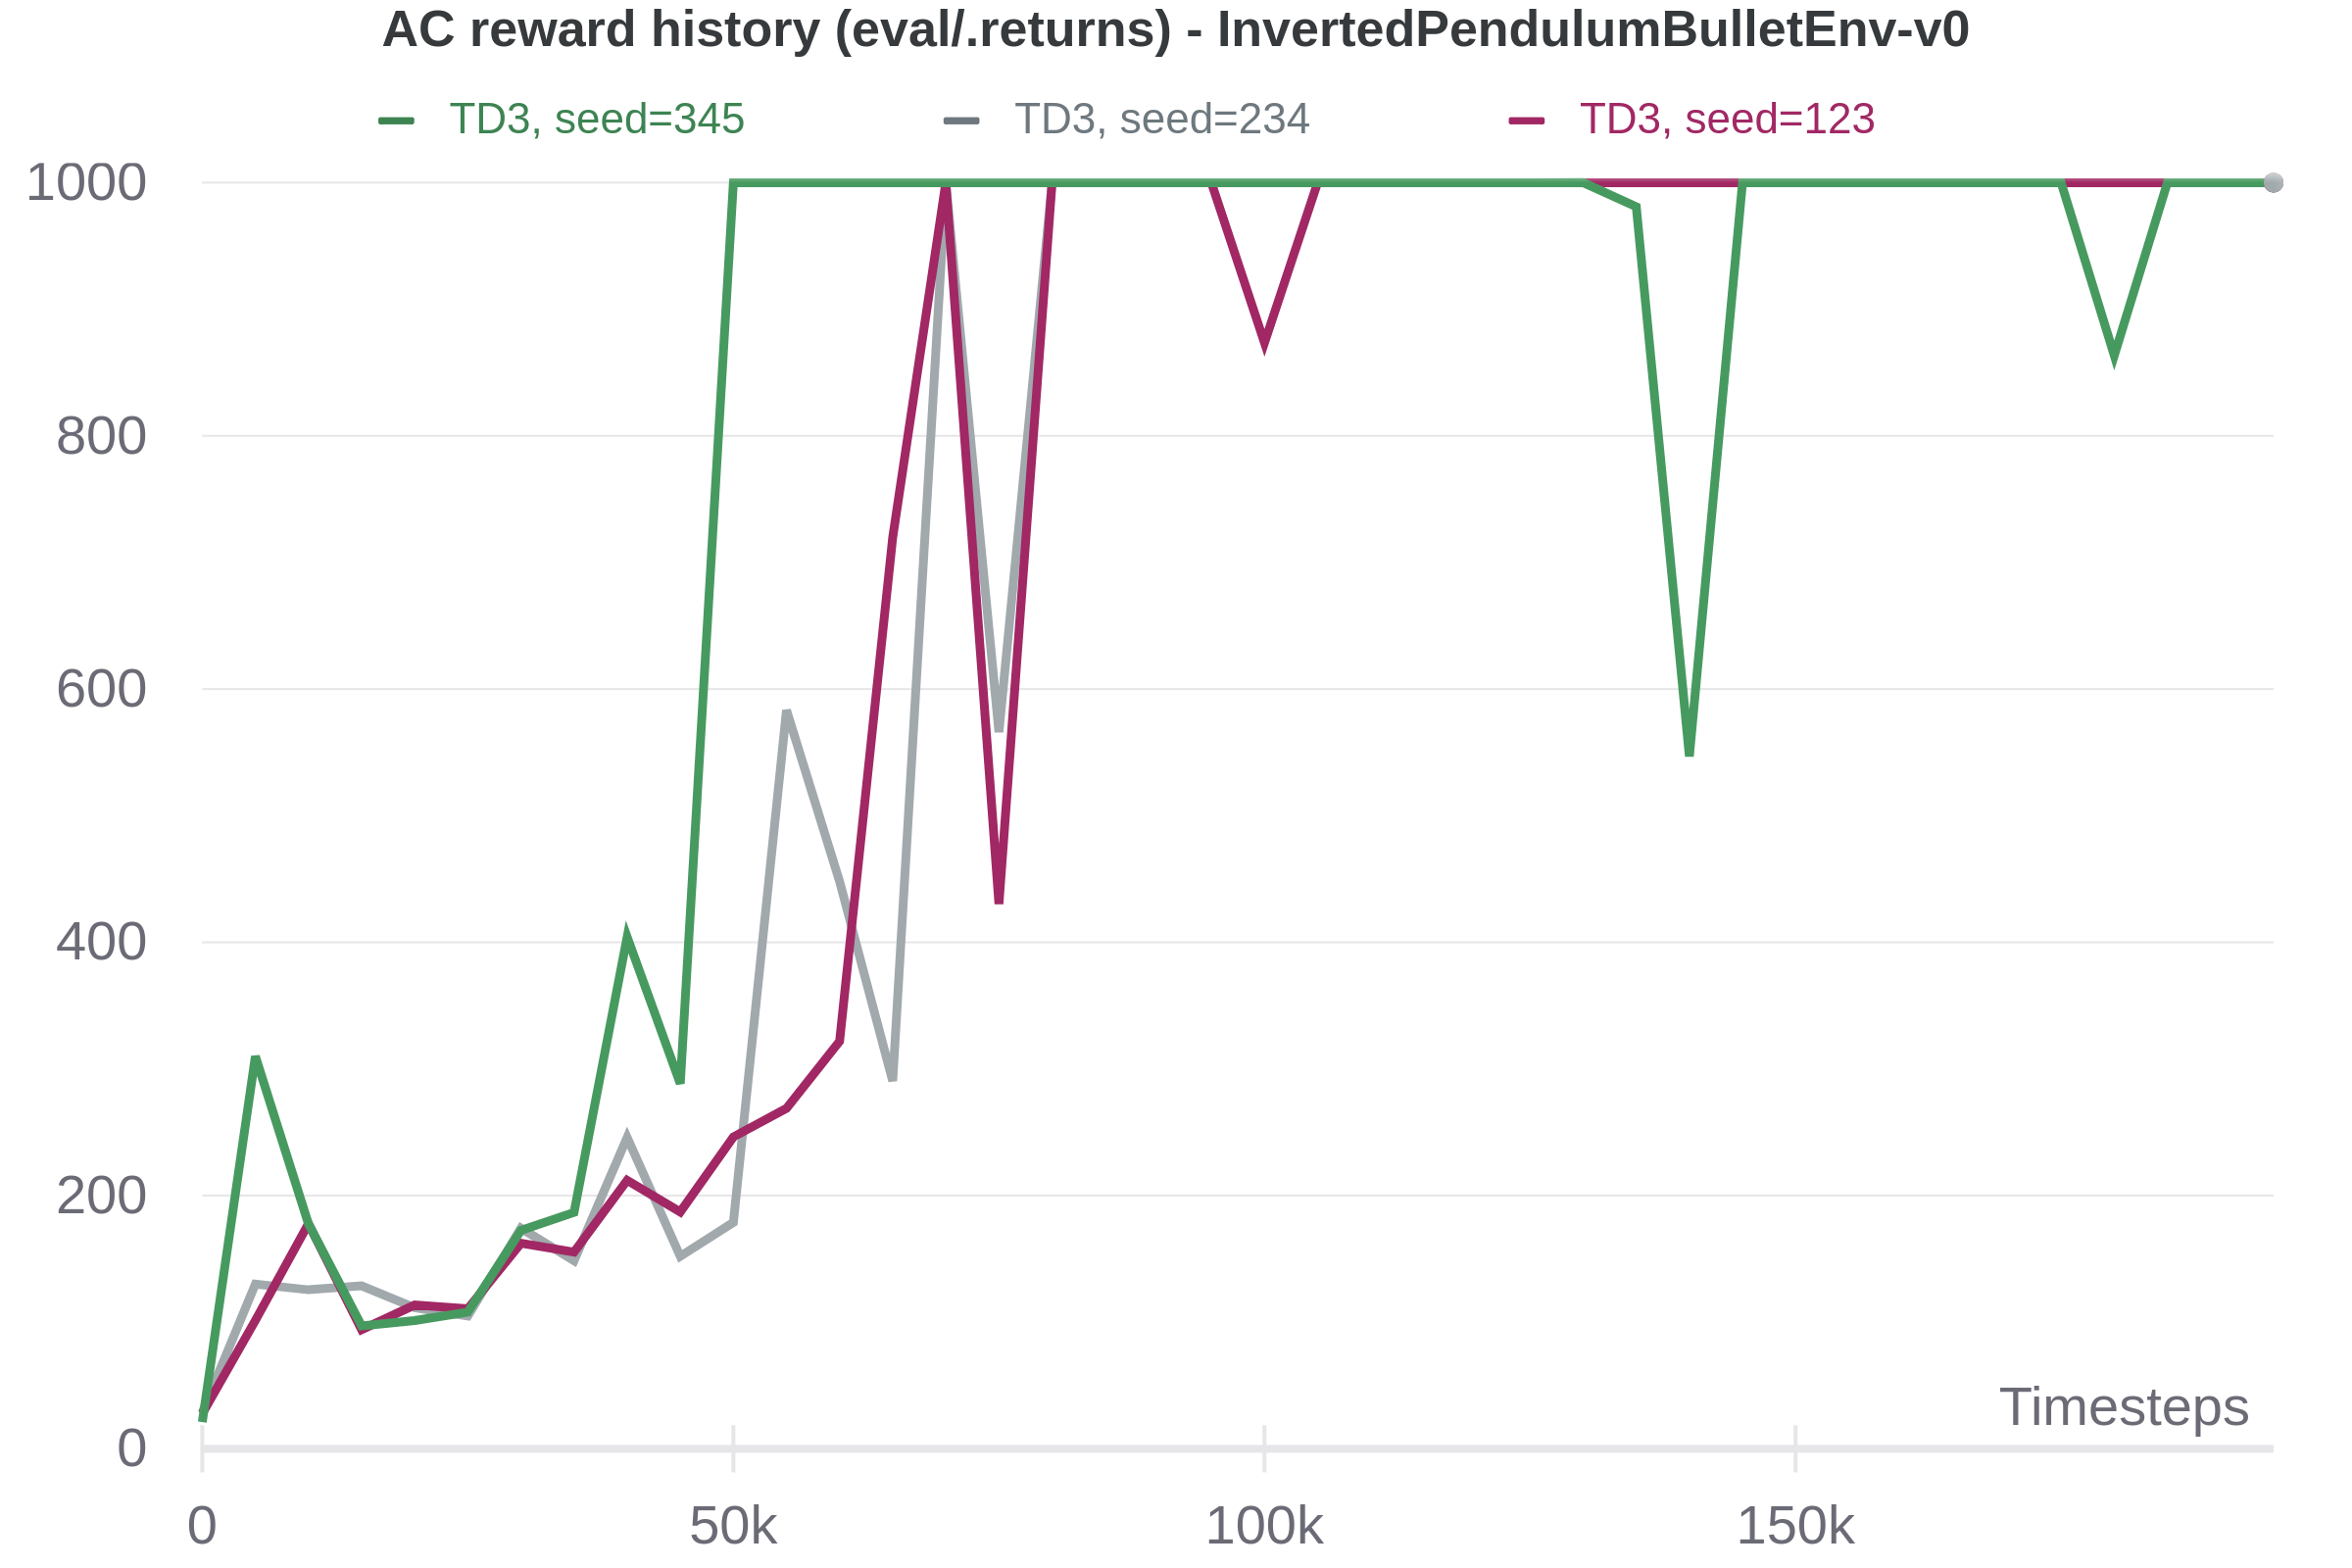
\includegraphics[width=0.65\columnwidth]{img/Figure_1_WB_InvertedPendulumBullet_TD3.png}
	\caption{Training performance of TD3 algorithm in InvertedPendulumBullet environment.}
	\label{fig:fig1}
\end{figure}

\begin{figure}[phb] 
	\centering  % Remember to centre the figure
    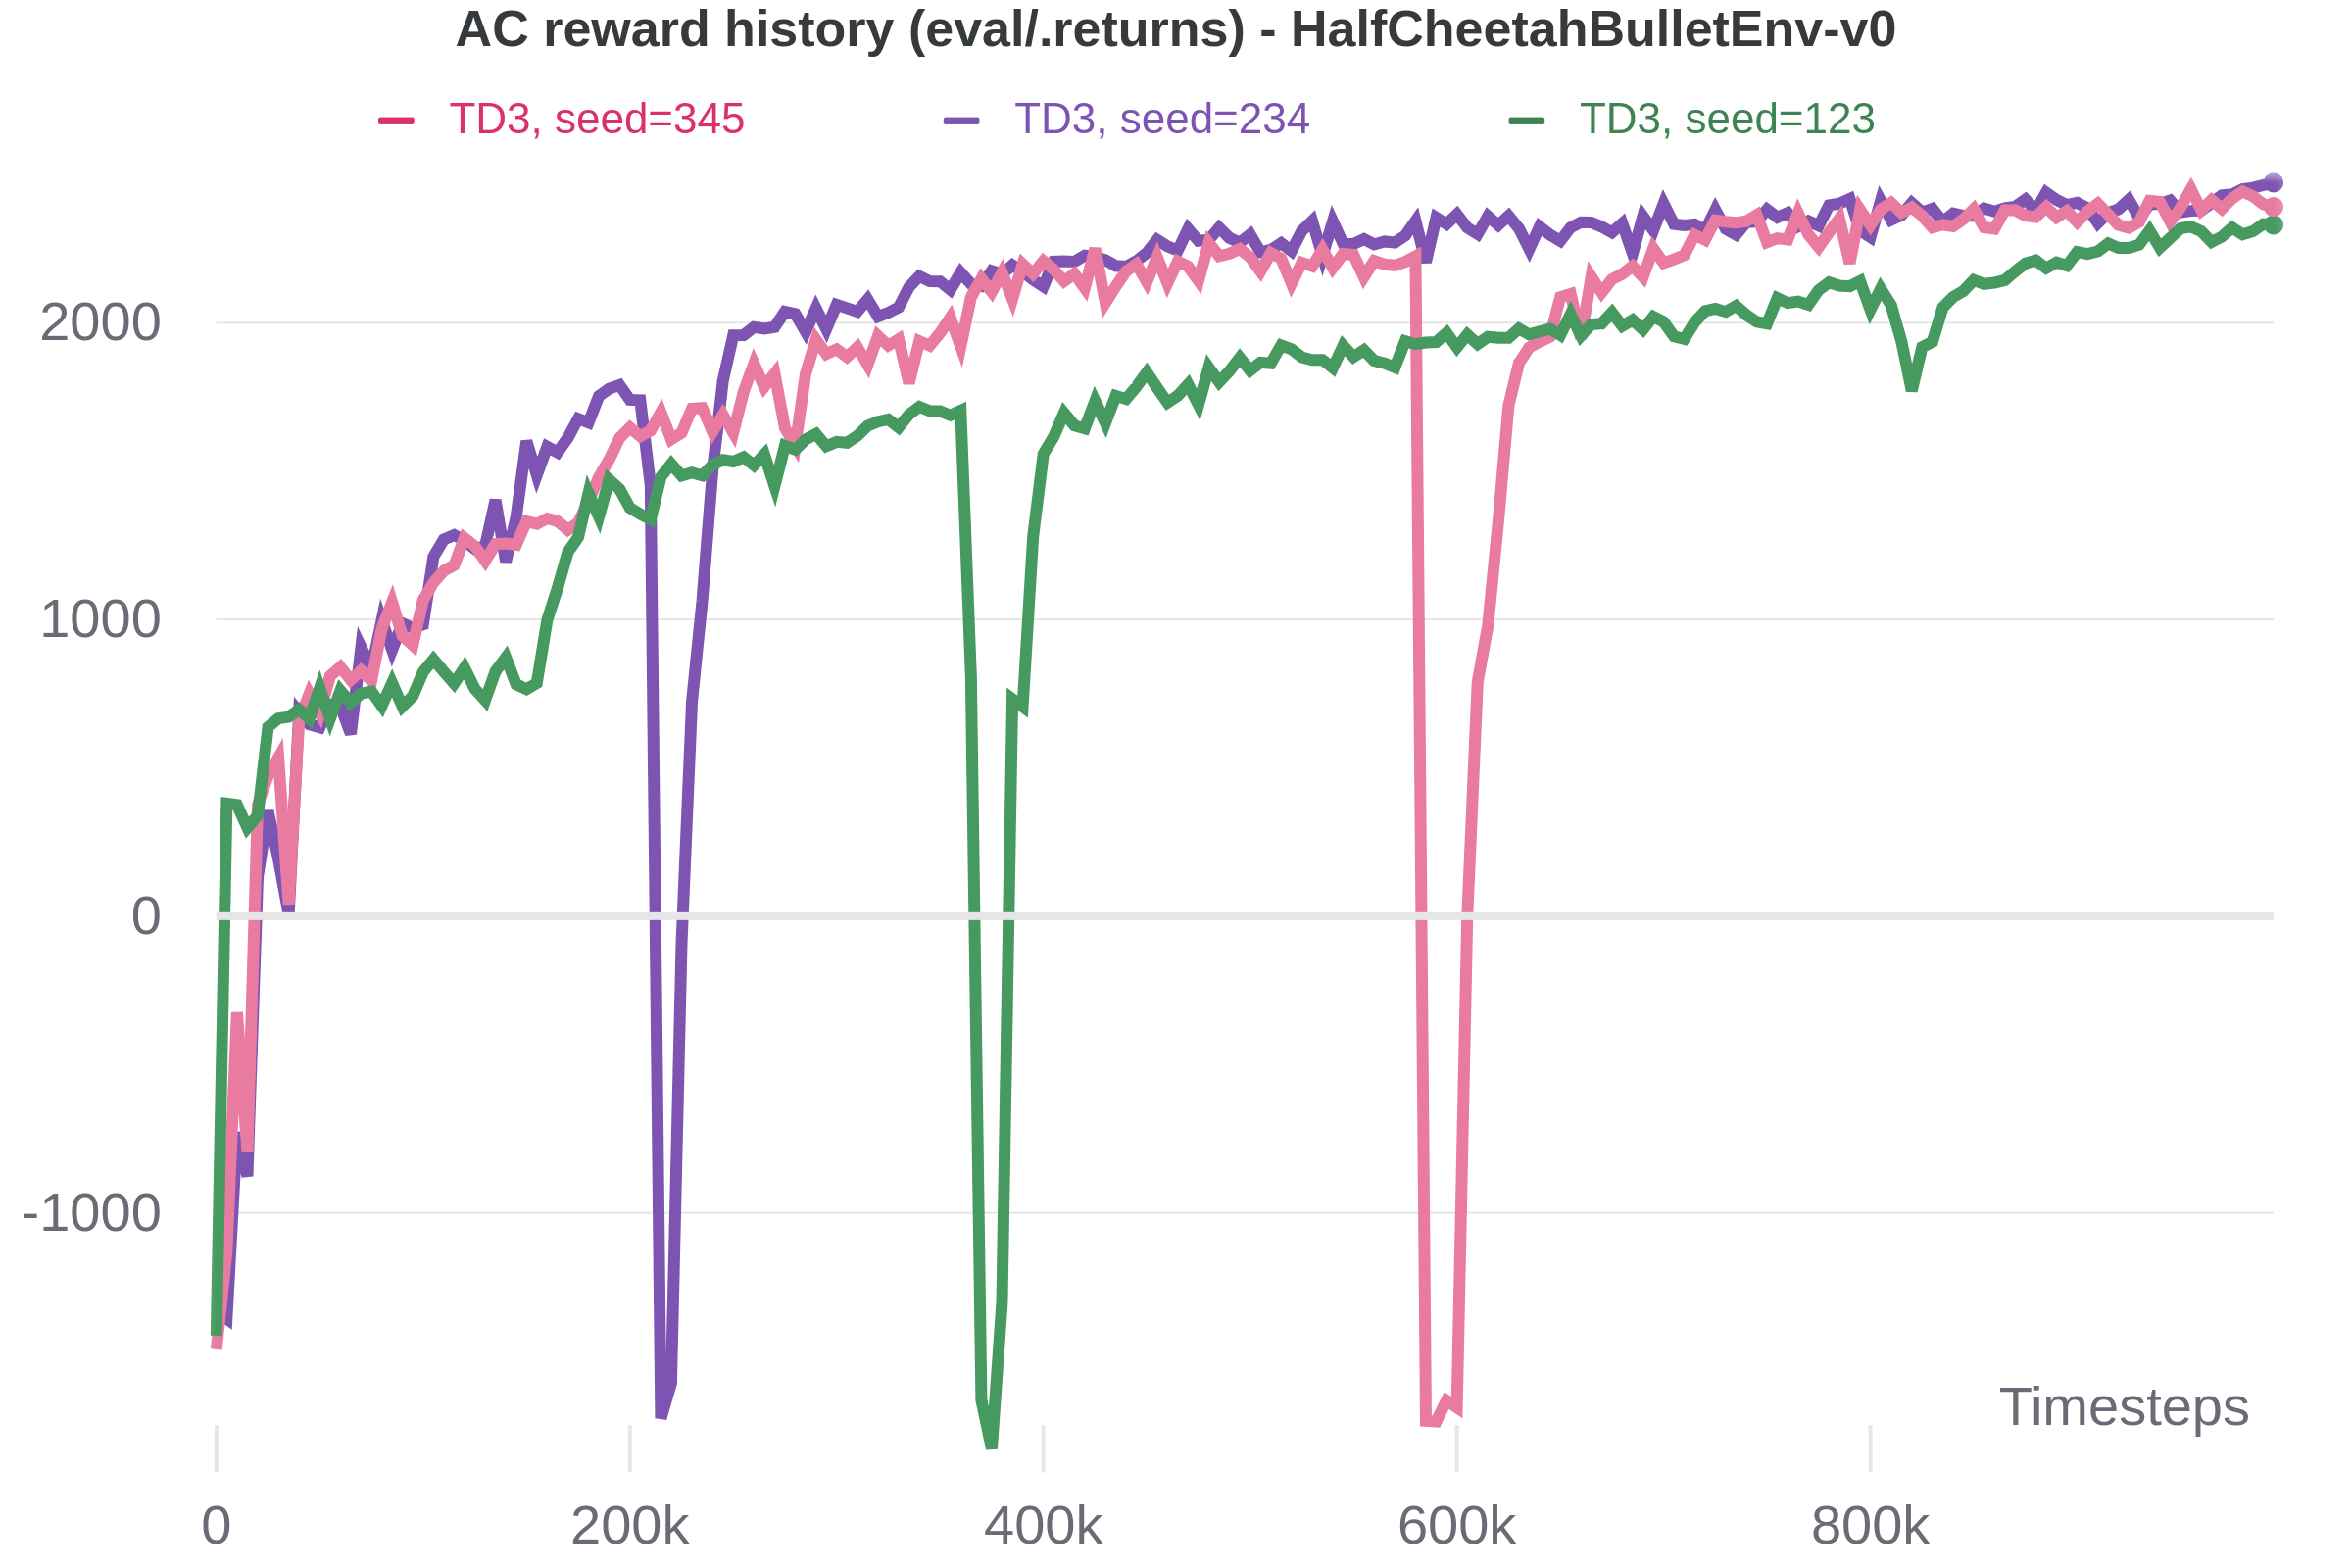
\includegraphics[width=0.65\columnwidth]{img/Figure_2_WB_HalfCheetahBullet_TD3.png}
	\caption{Training performance of TD3 algorithm in HalfCheetahBullet environment.}
	\label{fig:fig2}
\end{figure}

\pagebreak

\subsection*{Question 4}

Now let’s analyze the sensitivity of TD3 to hyperparameters. Choose one hyperparameter, e.g.,
target action noise, exploration noise, or policy update frequency, that you think heavily influence the training and explain why. Then, train your agent with the modified hyperparameter on both InvertedPendulumBulletEnv-v0 and HalfCheetahBulletEnv-v0 environments (3 random seeds).
Show the training plots and submit the trained model of HalfCheetah with name "td3\_q4.pth".

\subsection*{Question 5}

After playing with the TD3 algorithm, could you find any aspect that could be improved? Please
list three of them. Also, please propose a potential solution to one of the problems you listed.
You can answer this question by providing a paper link and explaining in your own words how
the proposed approach solves/mitigates the problem.

\pagebreak

\subsection*{Algorithm 2: Proximal Policy Optimization Algorithms (PPO)}

\subsection*{Question 1}

Why does clipping the $\dfrac{\pi_{\theta}(a|s)}{\pi_{old}(a|s)}$ ratio stabilize the training? What is the relationship between TRPO [7] and PPO?

\subsection*{Question 2}

Please finish the implementation of the PPO algorithm.
\newline

\noindent
Similar to Question 3, train the agent on both the InvertedPendulumBulletEnv-v0 and the HalfCheetahBulletEnv-v0 environments.
\newline

\noindent
Train your agents with three random seeds for both environments. 
\newline

\noindent
Include the training plots in the project report and attach the agents’ weights to your submission, with filenames ending with ppo.pth containing the run ID (1, 2, and 3, each with a different random seed) and the environment name. 
\newline

\noindent
For the training curve, you can reference 2. 


Training performance of PPO algorithm in InvertedPendulumBullet environment is presented in Figure.~\ref*{fig:fig3}.
\newline

Training performance of PPO algorithm in HalfCheetahBullet environment is presented in Figure.~\ref*{fig:fig4}.
\newline


\pagebreak

\begin{figure}[pht] 
	\centering  % Remember to centre the figure
    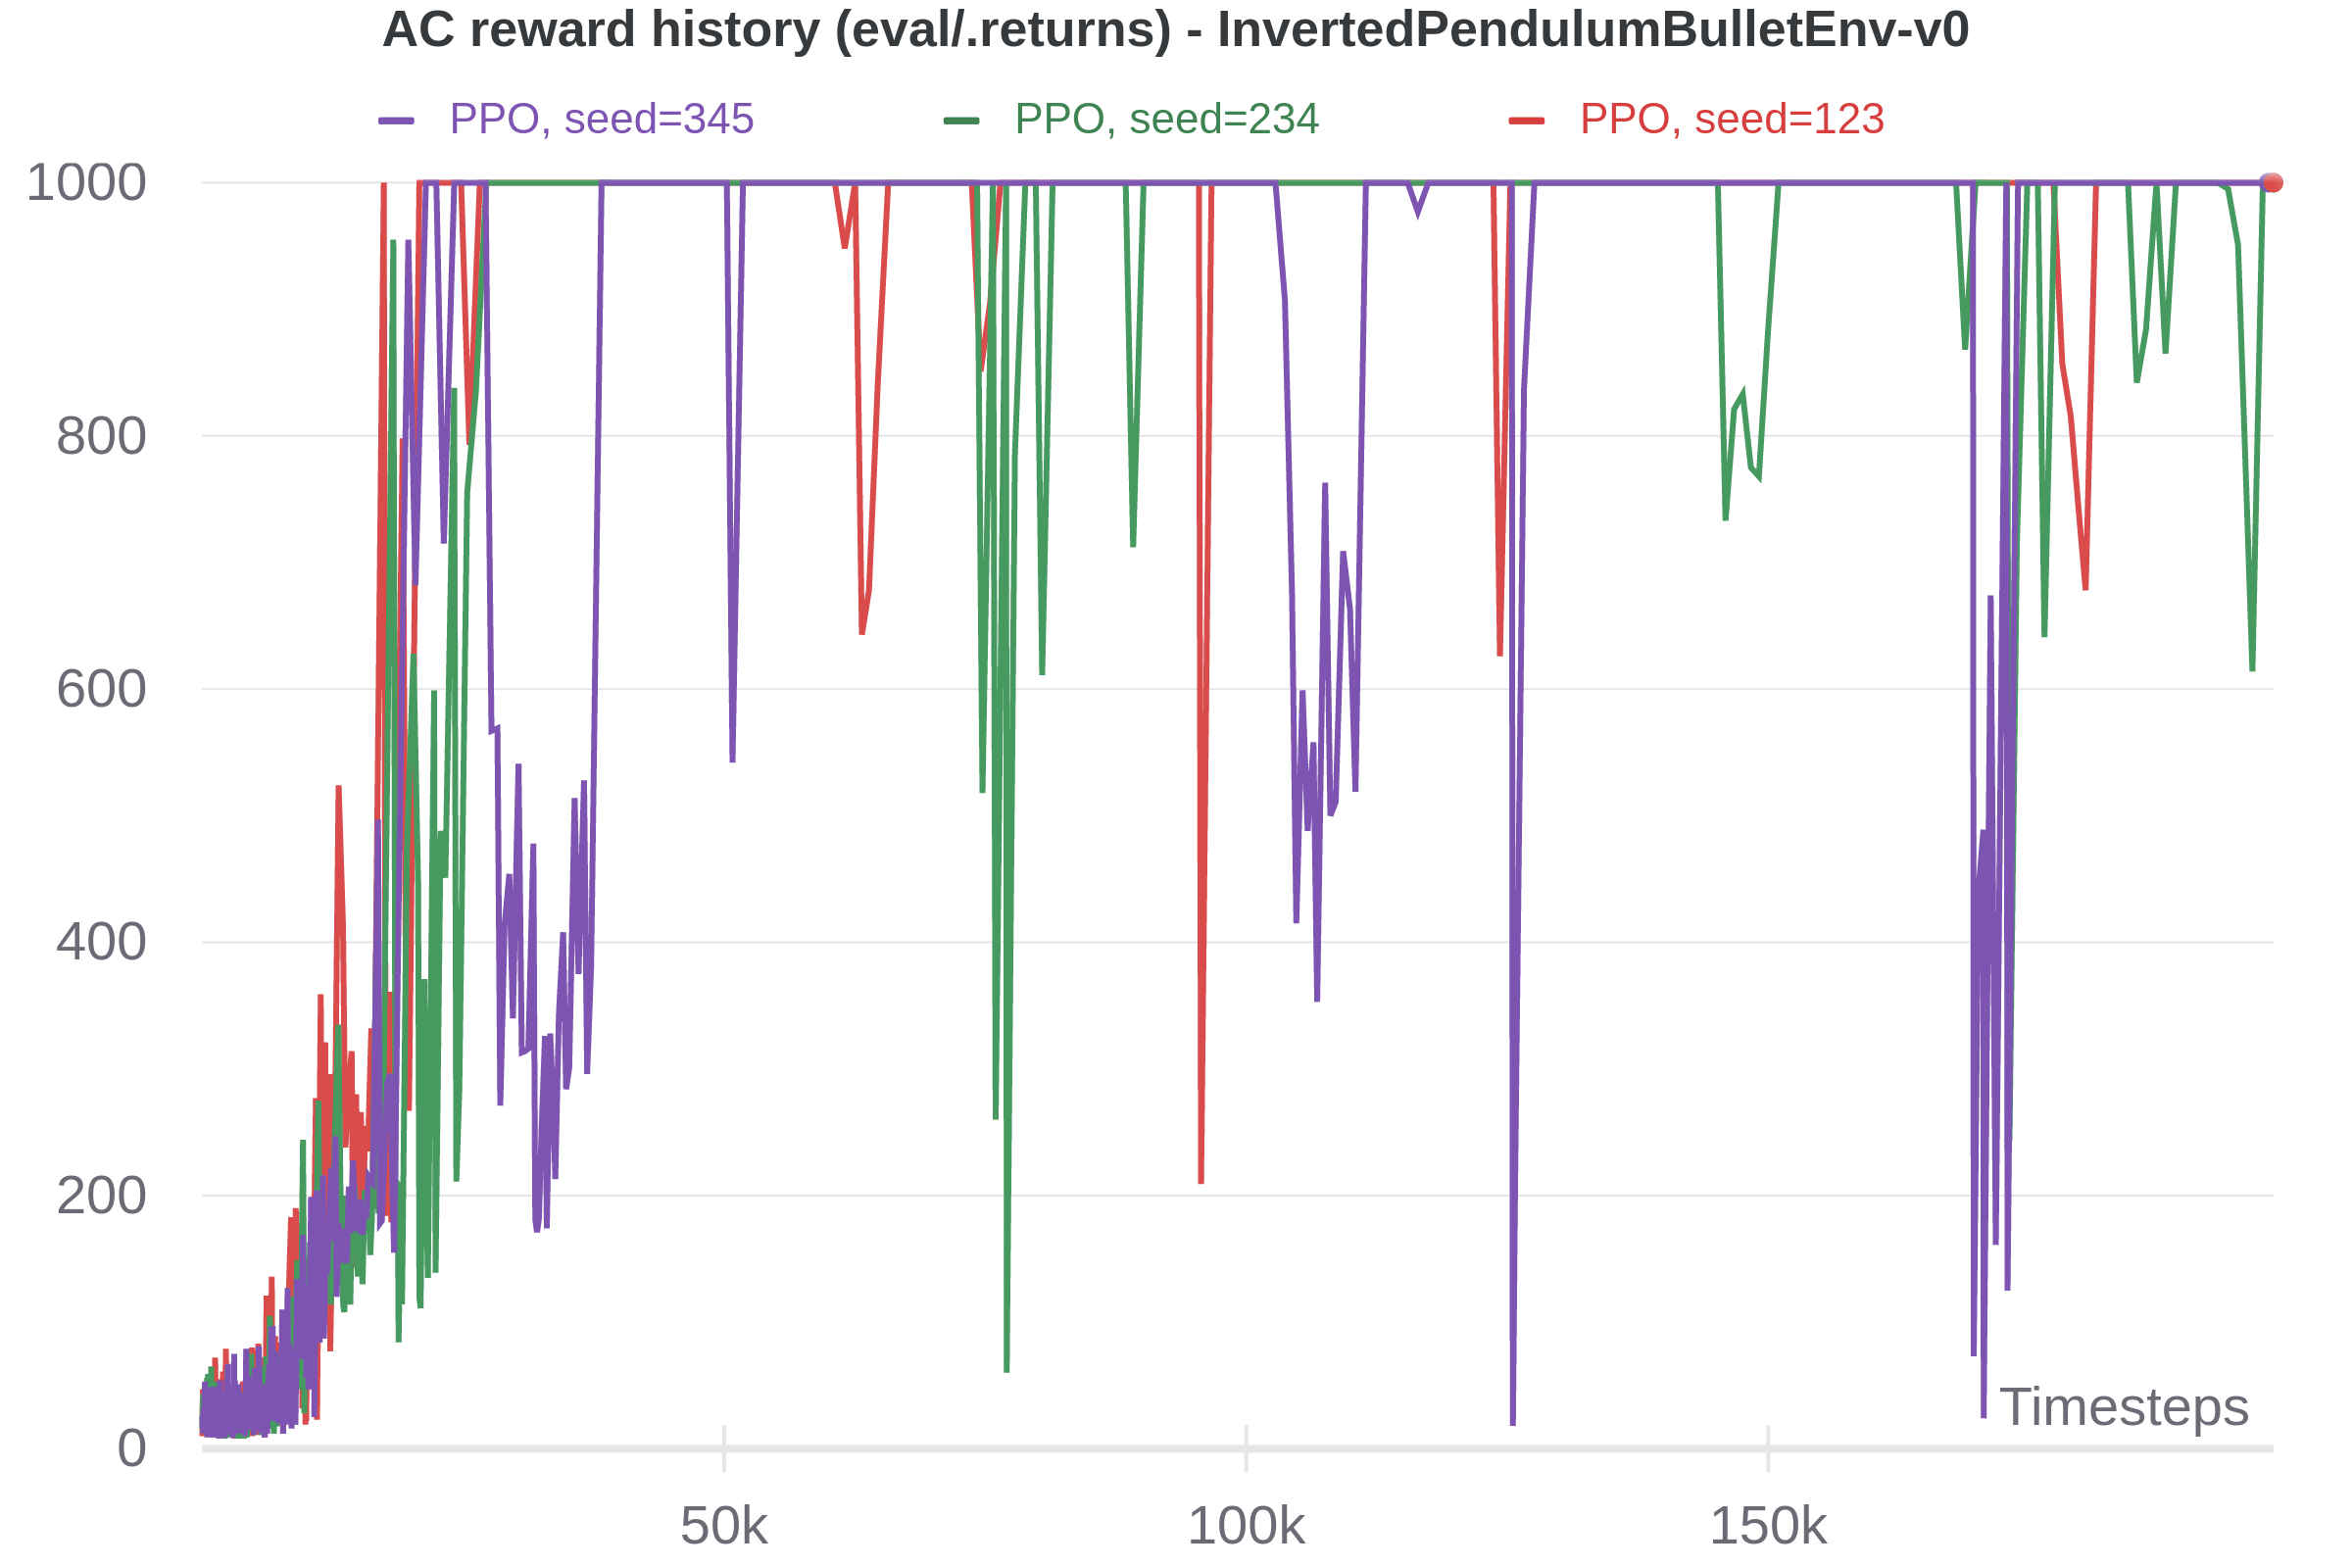
\includegraphics[width=0.65\columnwidth]{img/Figure_3_WB_InvertedPendulumBullet_PPO.png}
	\caption{Training performance of PPO algorithm in InvertedPendulumBullet environment.}
	\label{fig:fig3}
\end{figure}

\begin{figure}[phb] 
	\centering  % Remember to centre the figure
    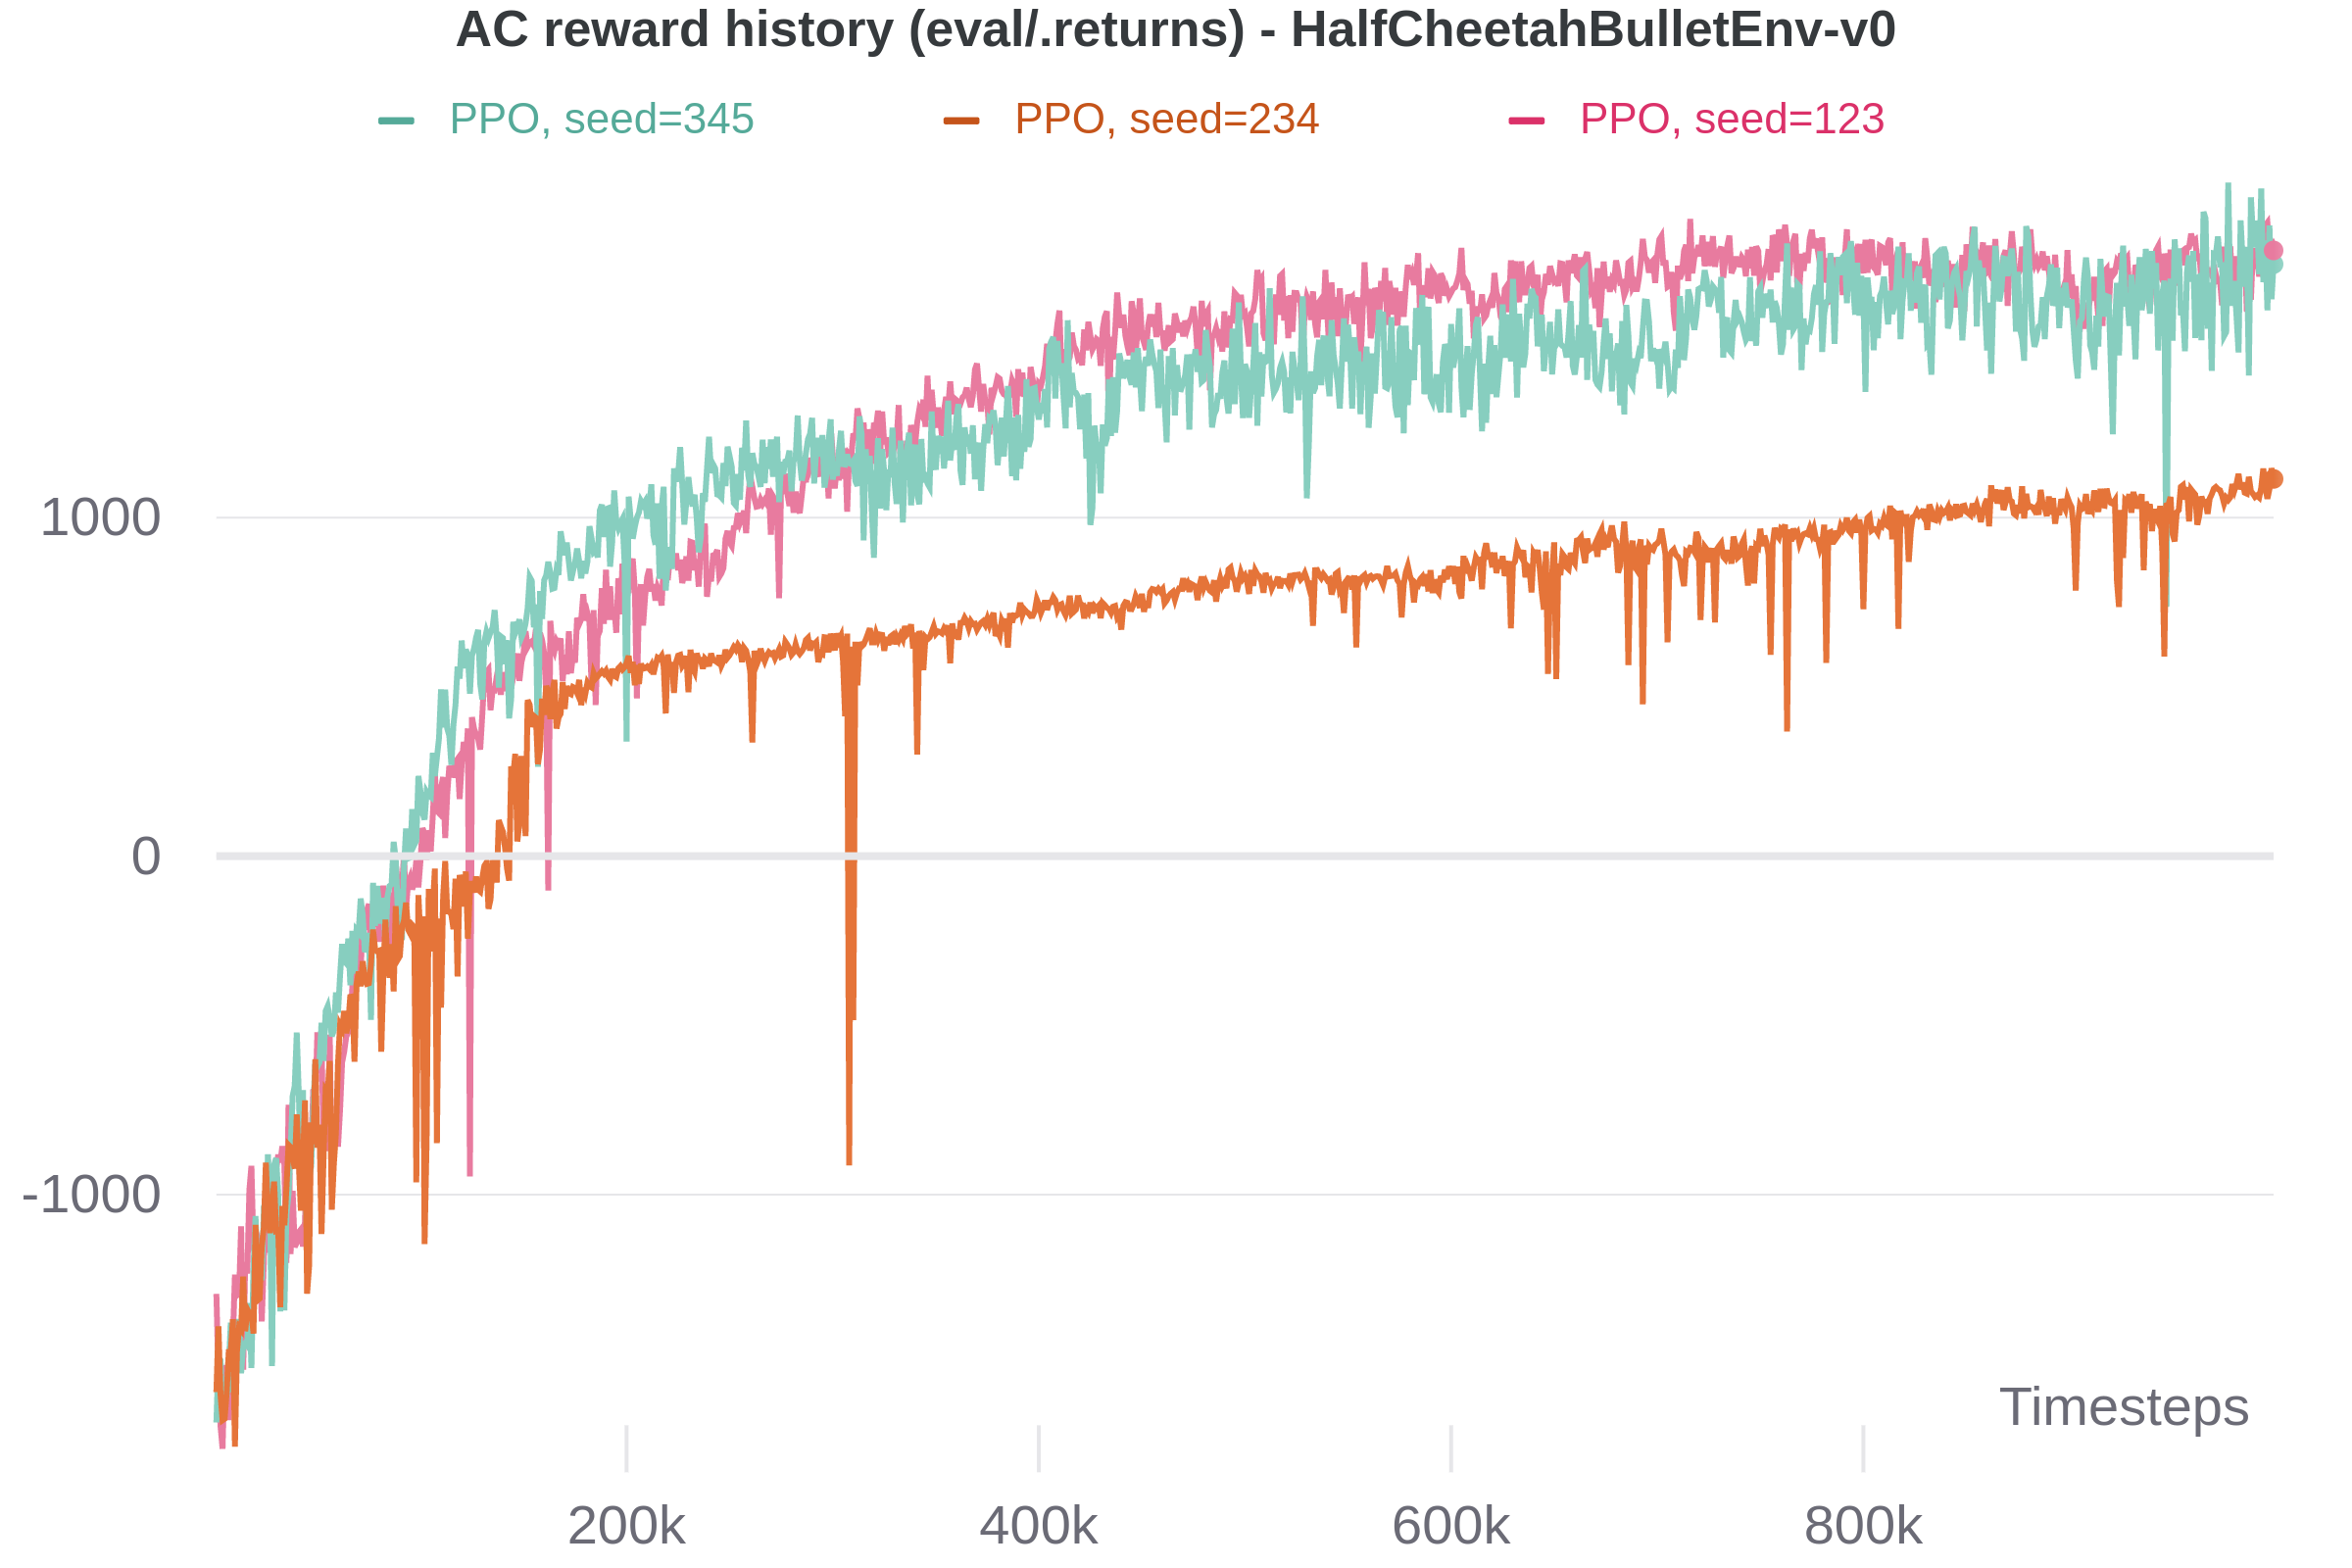
\includegraphics[width=0.65\columnwidth]{img/Figure_4_WB_HalfCheetahBullet_PPO.png}
	\caption{Training performance of PPO algorithm in HalfCheetahBullet environment.}
	\label{fig:fig4}
\end{figure}

\pagebreak

\subsection*{Question 3}

In PPO, the target value is calculated by generalized advantage estimation (GAE) [8], 
as shown in the second equation. Explain the relationship between n-step advantage and GAE. 
Why is GAE better than n-step advantage?

\pagebreak



\section*{Part 2}

Answers to the questions in part 2.
\newline

\subsection*{Question 1}

\noindent
Please correctly implement your algorithm and show the training plots against the TD3/PPO
with three random seeds. 
\newline

\noindent
The plots should include both InvertedPendulum and HalfCheetah environments. 
\newline


Training performance of SAC algorithm in InvertedPendulumBullet environment is presented in Figure.~\ref*{fig:fig5}.
\newline

Training performance of SAC algorithm in HalfCheetahBullet environment is presented in Figure.~\ref*{fig:fig6}.
\newline


\pagebreak

\begin{figure}[pht] 
	\centering  % Remember to centre the figure
    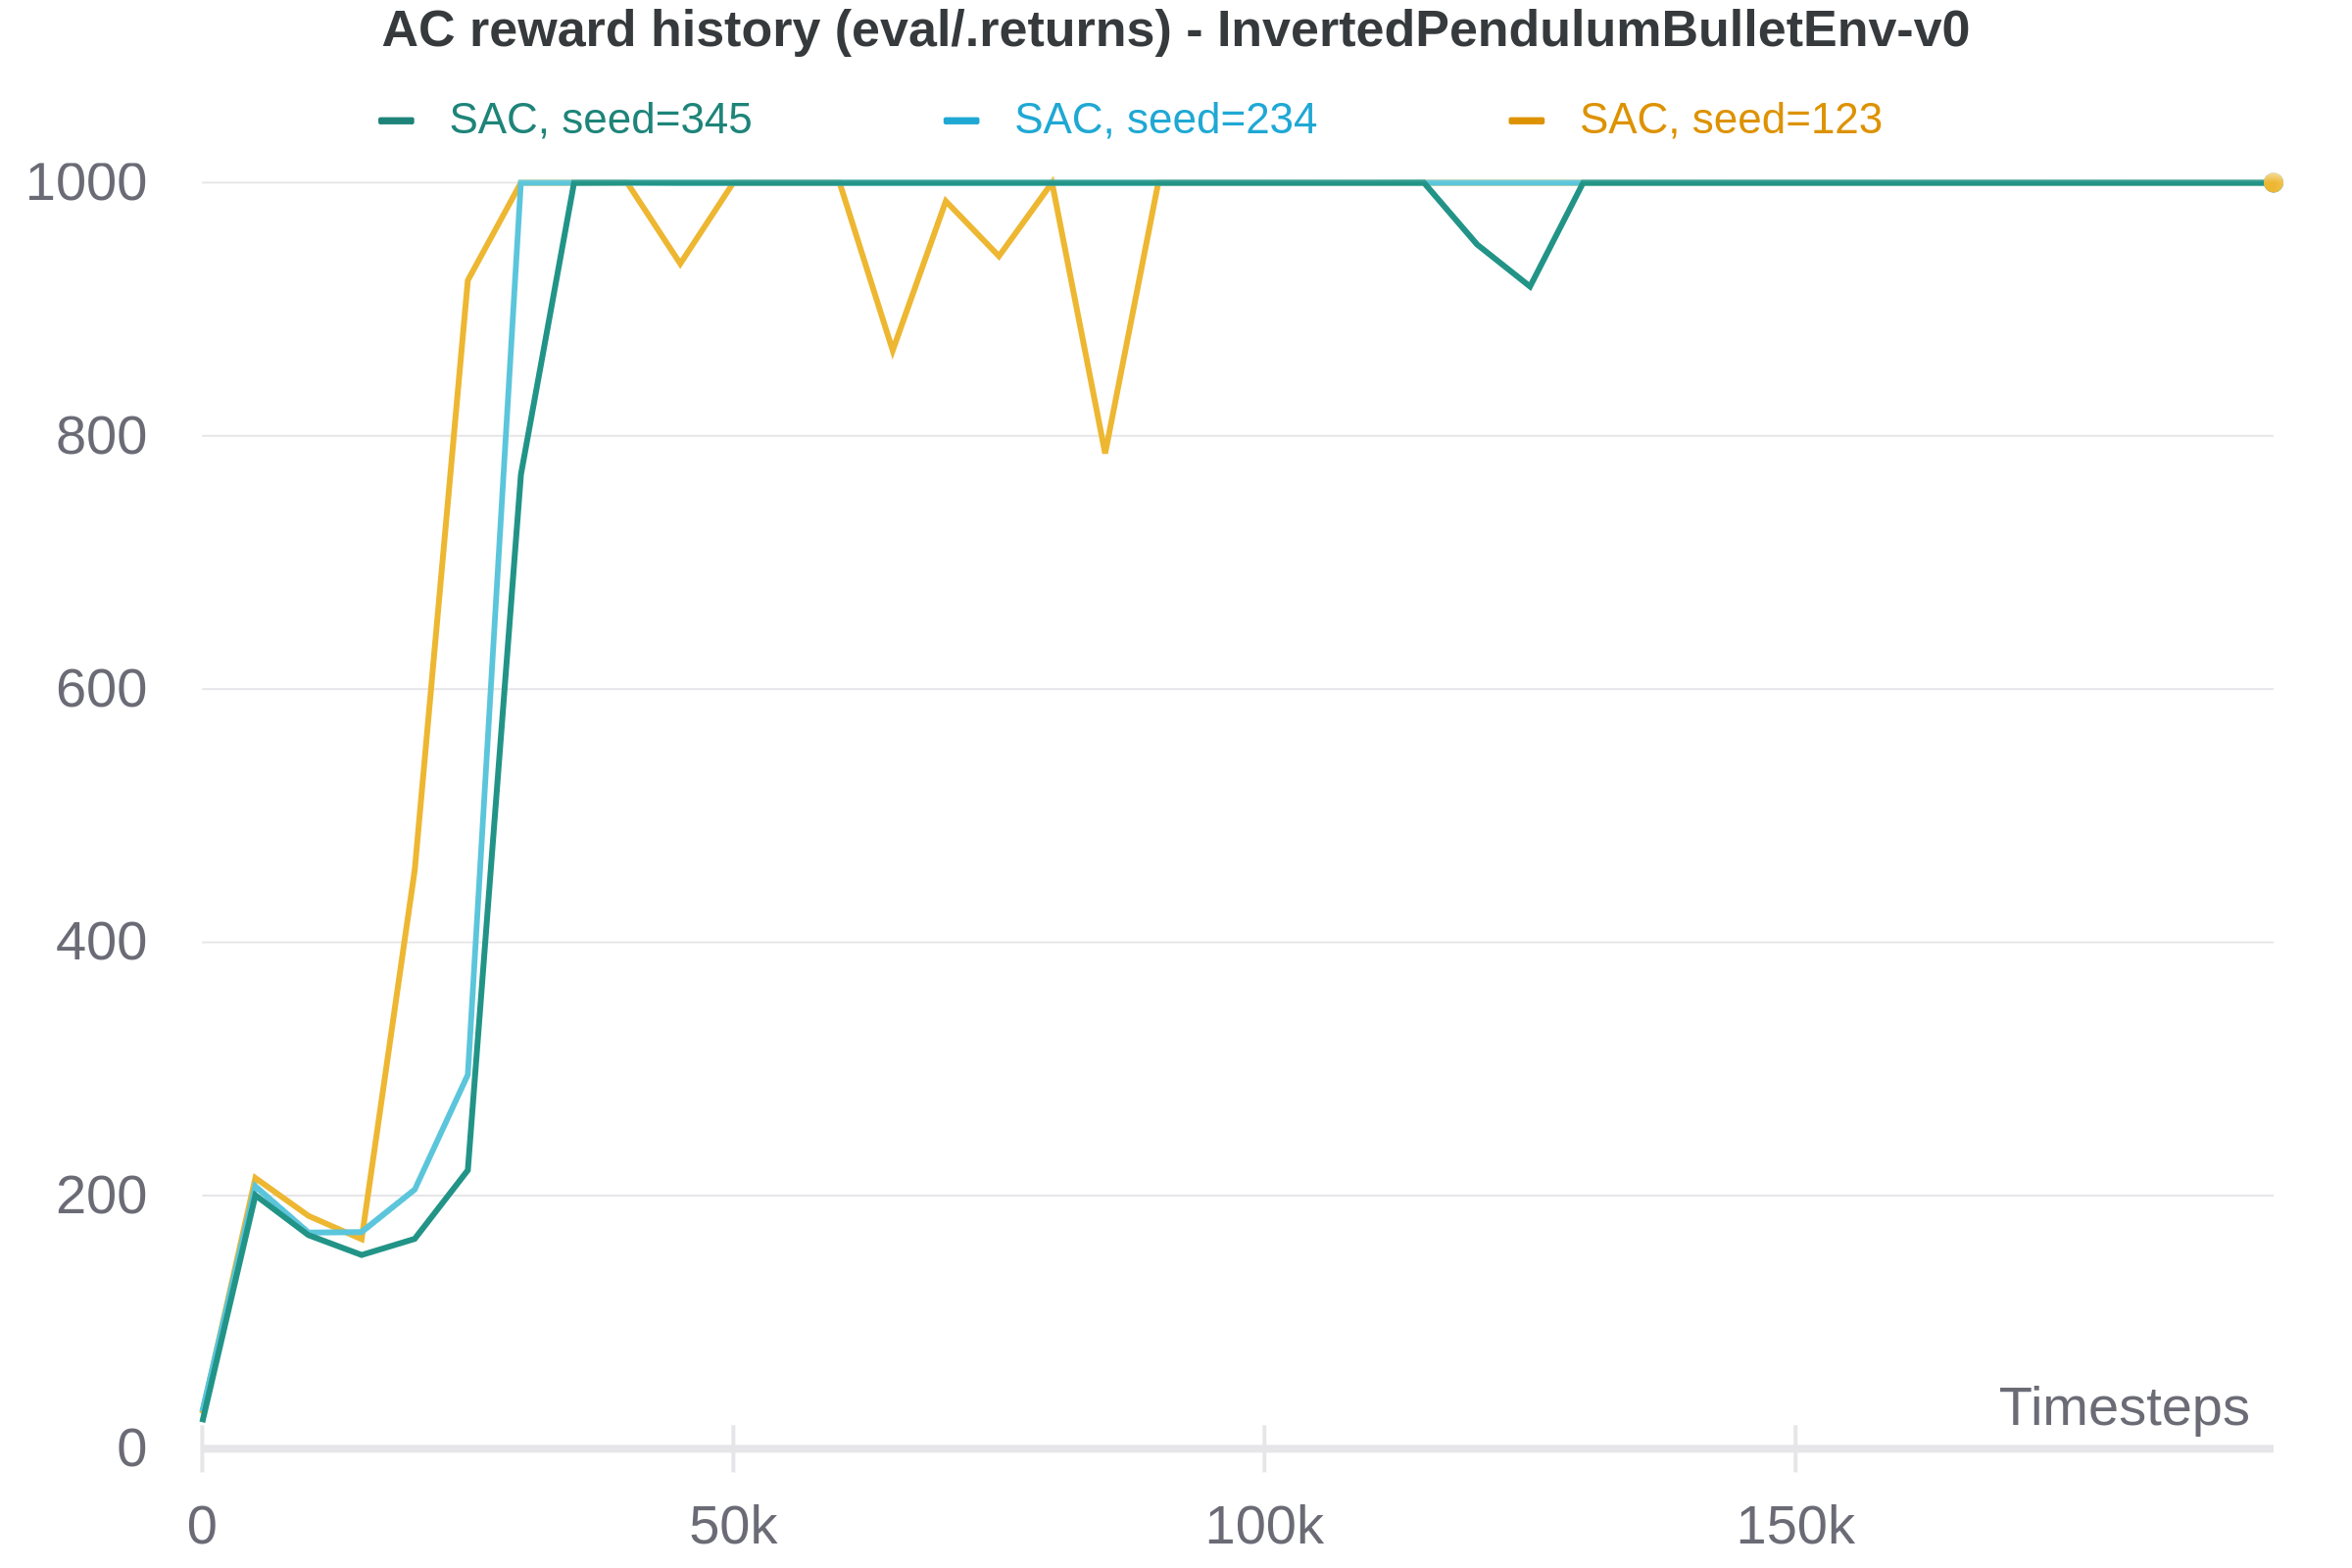
\includegraphics[width=0.65\columnwidth]{img/Figure_5_WB_InvertedPendulumBullet_SAC.png}
	\caption{OLD: Training performance of SAC algorithm in InvertedPendulumBullet environment.}
	\label{fig:fig5}
\end{figure}

\begin{figure}[phb] 
	\centering  % Remember to centre the figure
    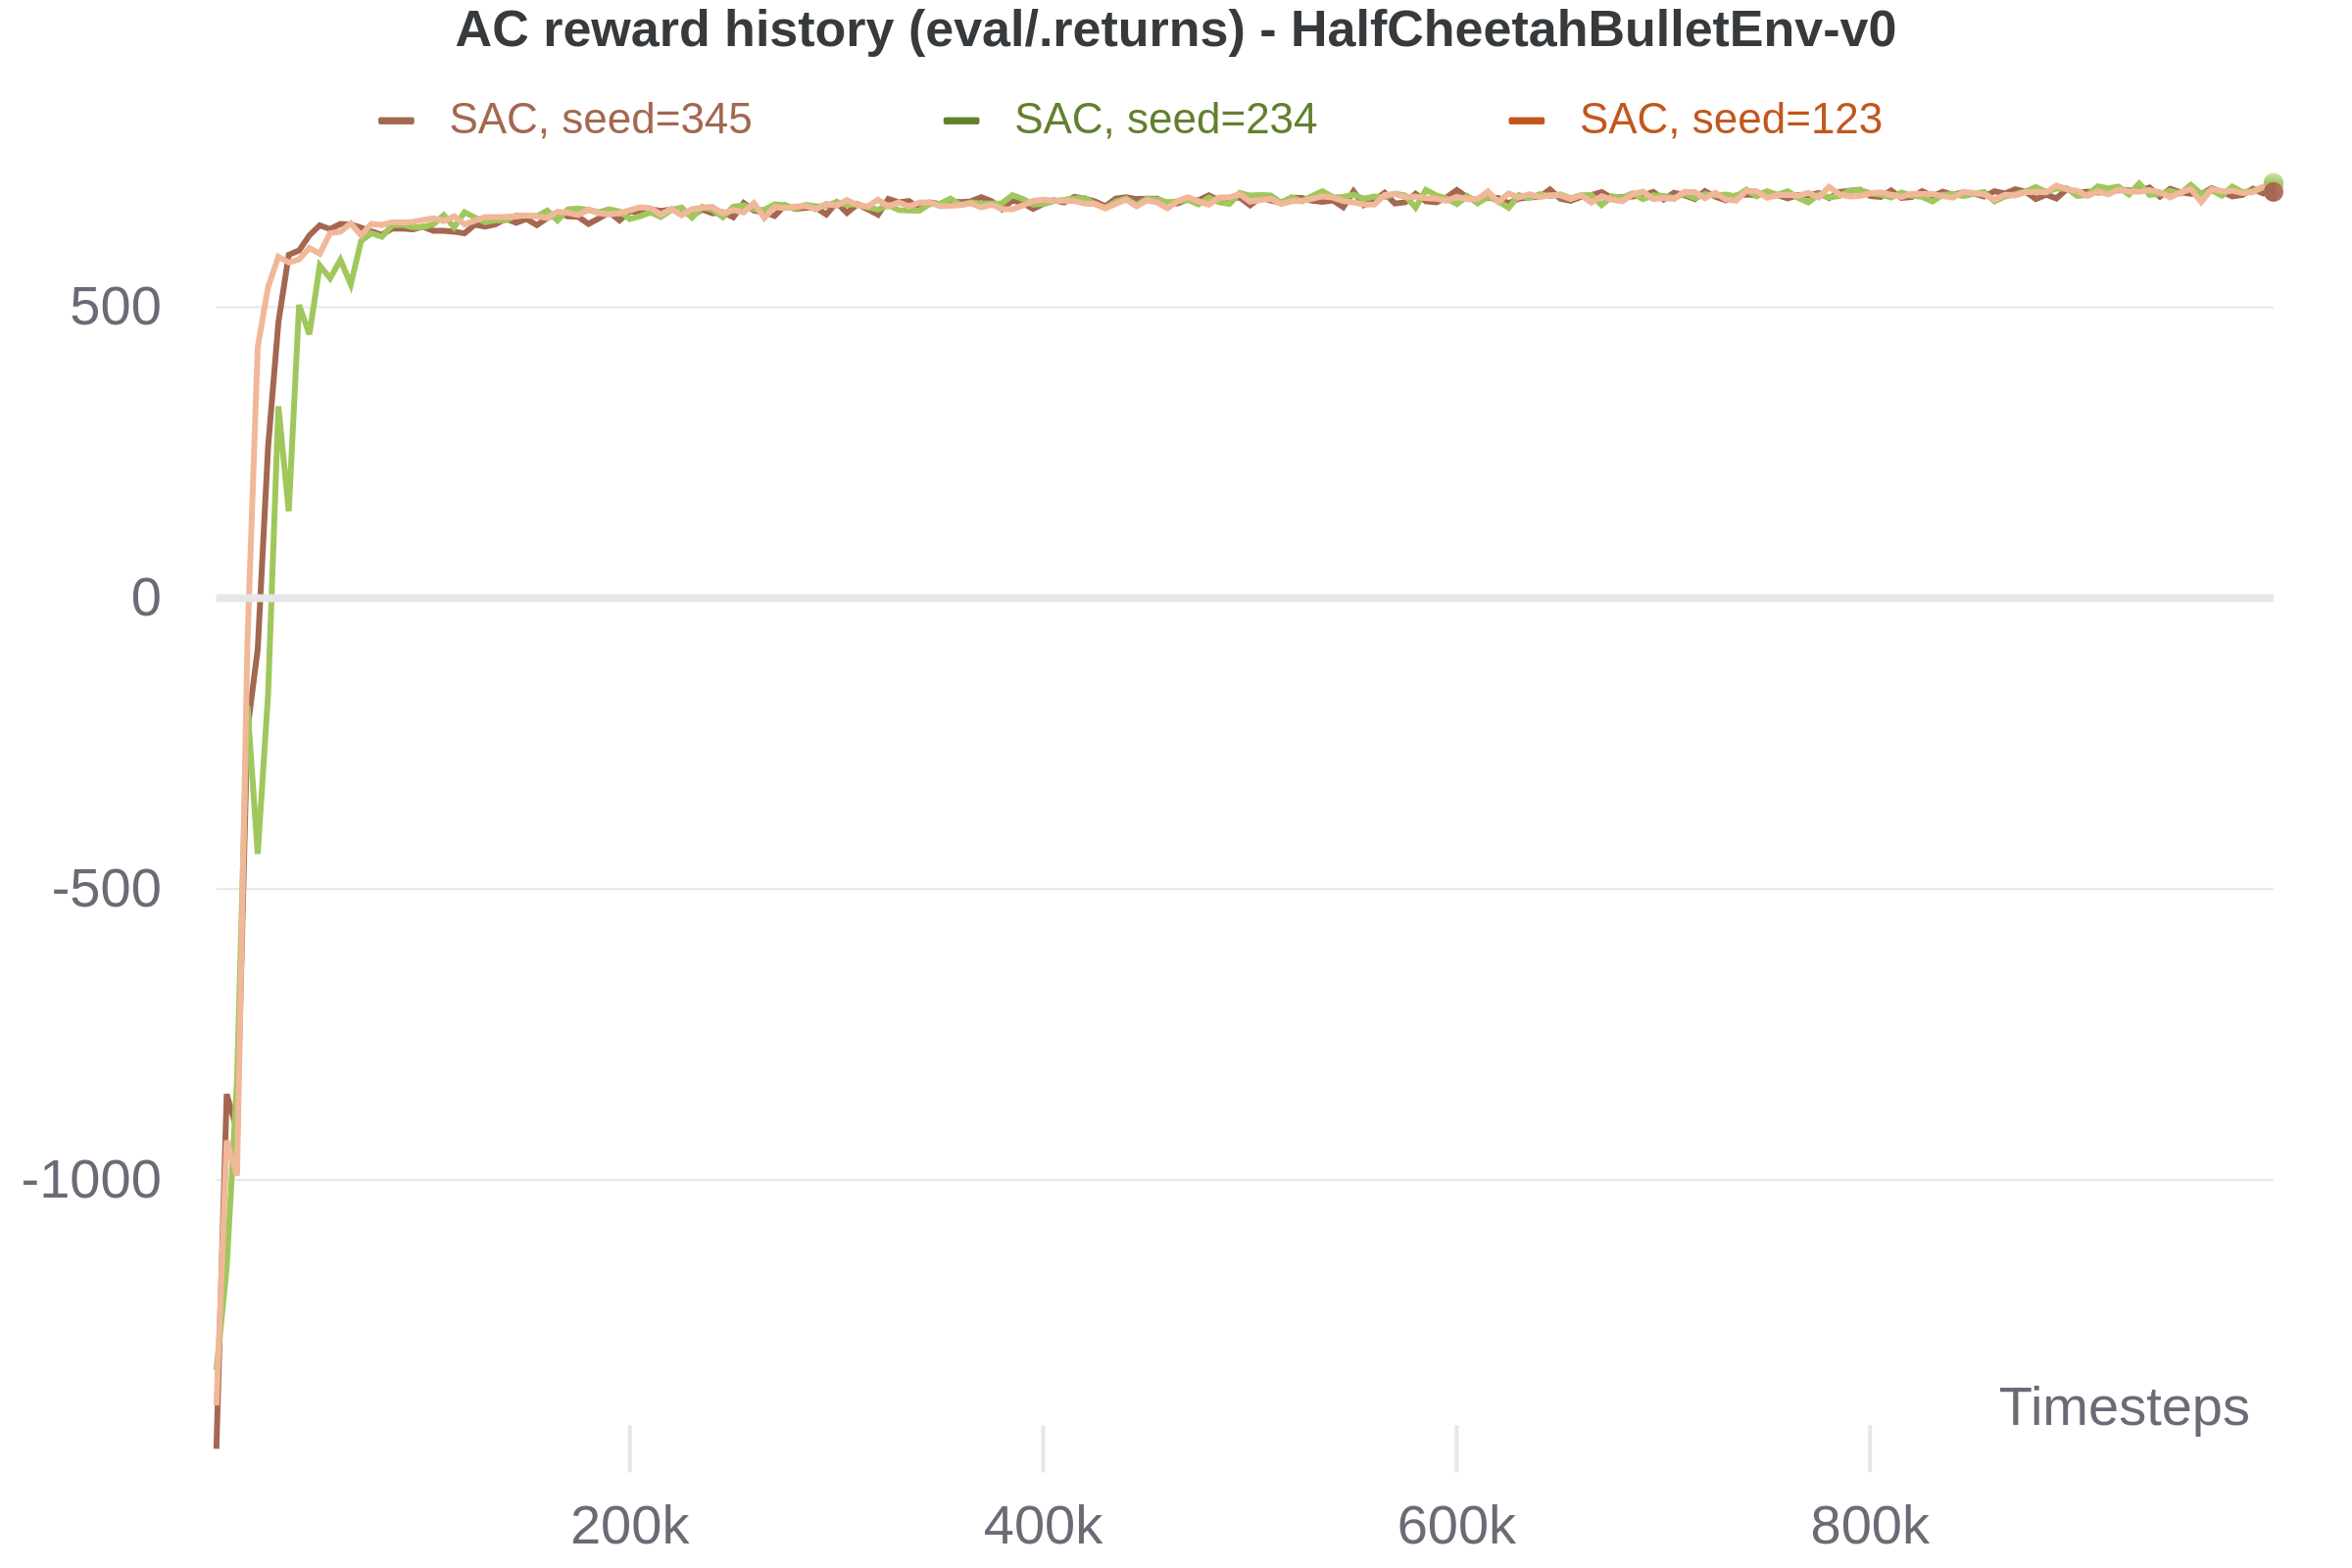
\includegraphics[width=0.65\columnwidth]{img/Figure_6_WB_HalfCheetahBullet_SAC.png}
	\caption{OLD: Training performance of SAC algorithm in HalfCheetahBullet environment.}
	\label{fig:fig6}
\end{figure}

\pagebreak

\begin{figure}[pht] 
	\centering  % Remember to centre the figure
    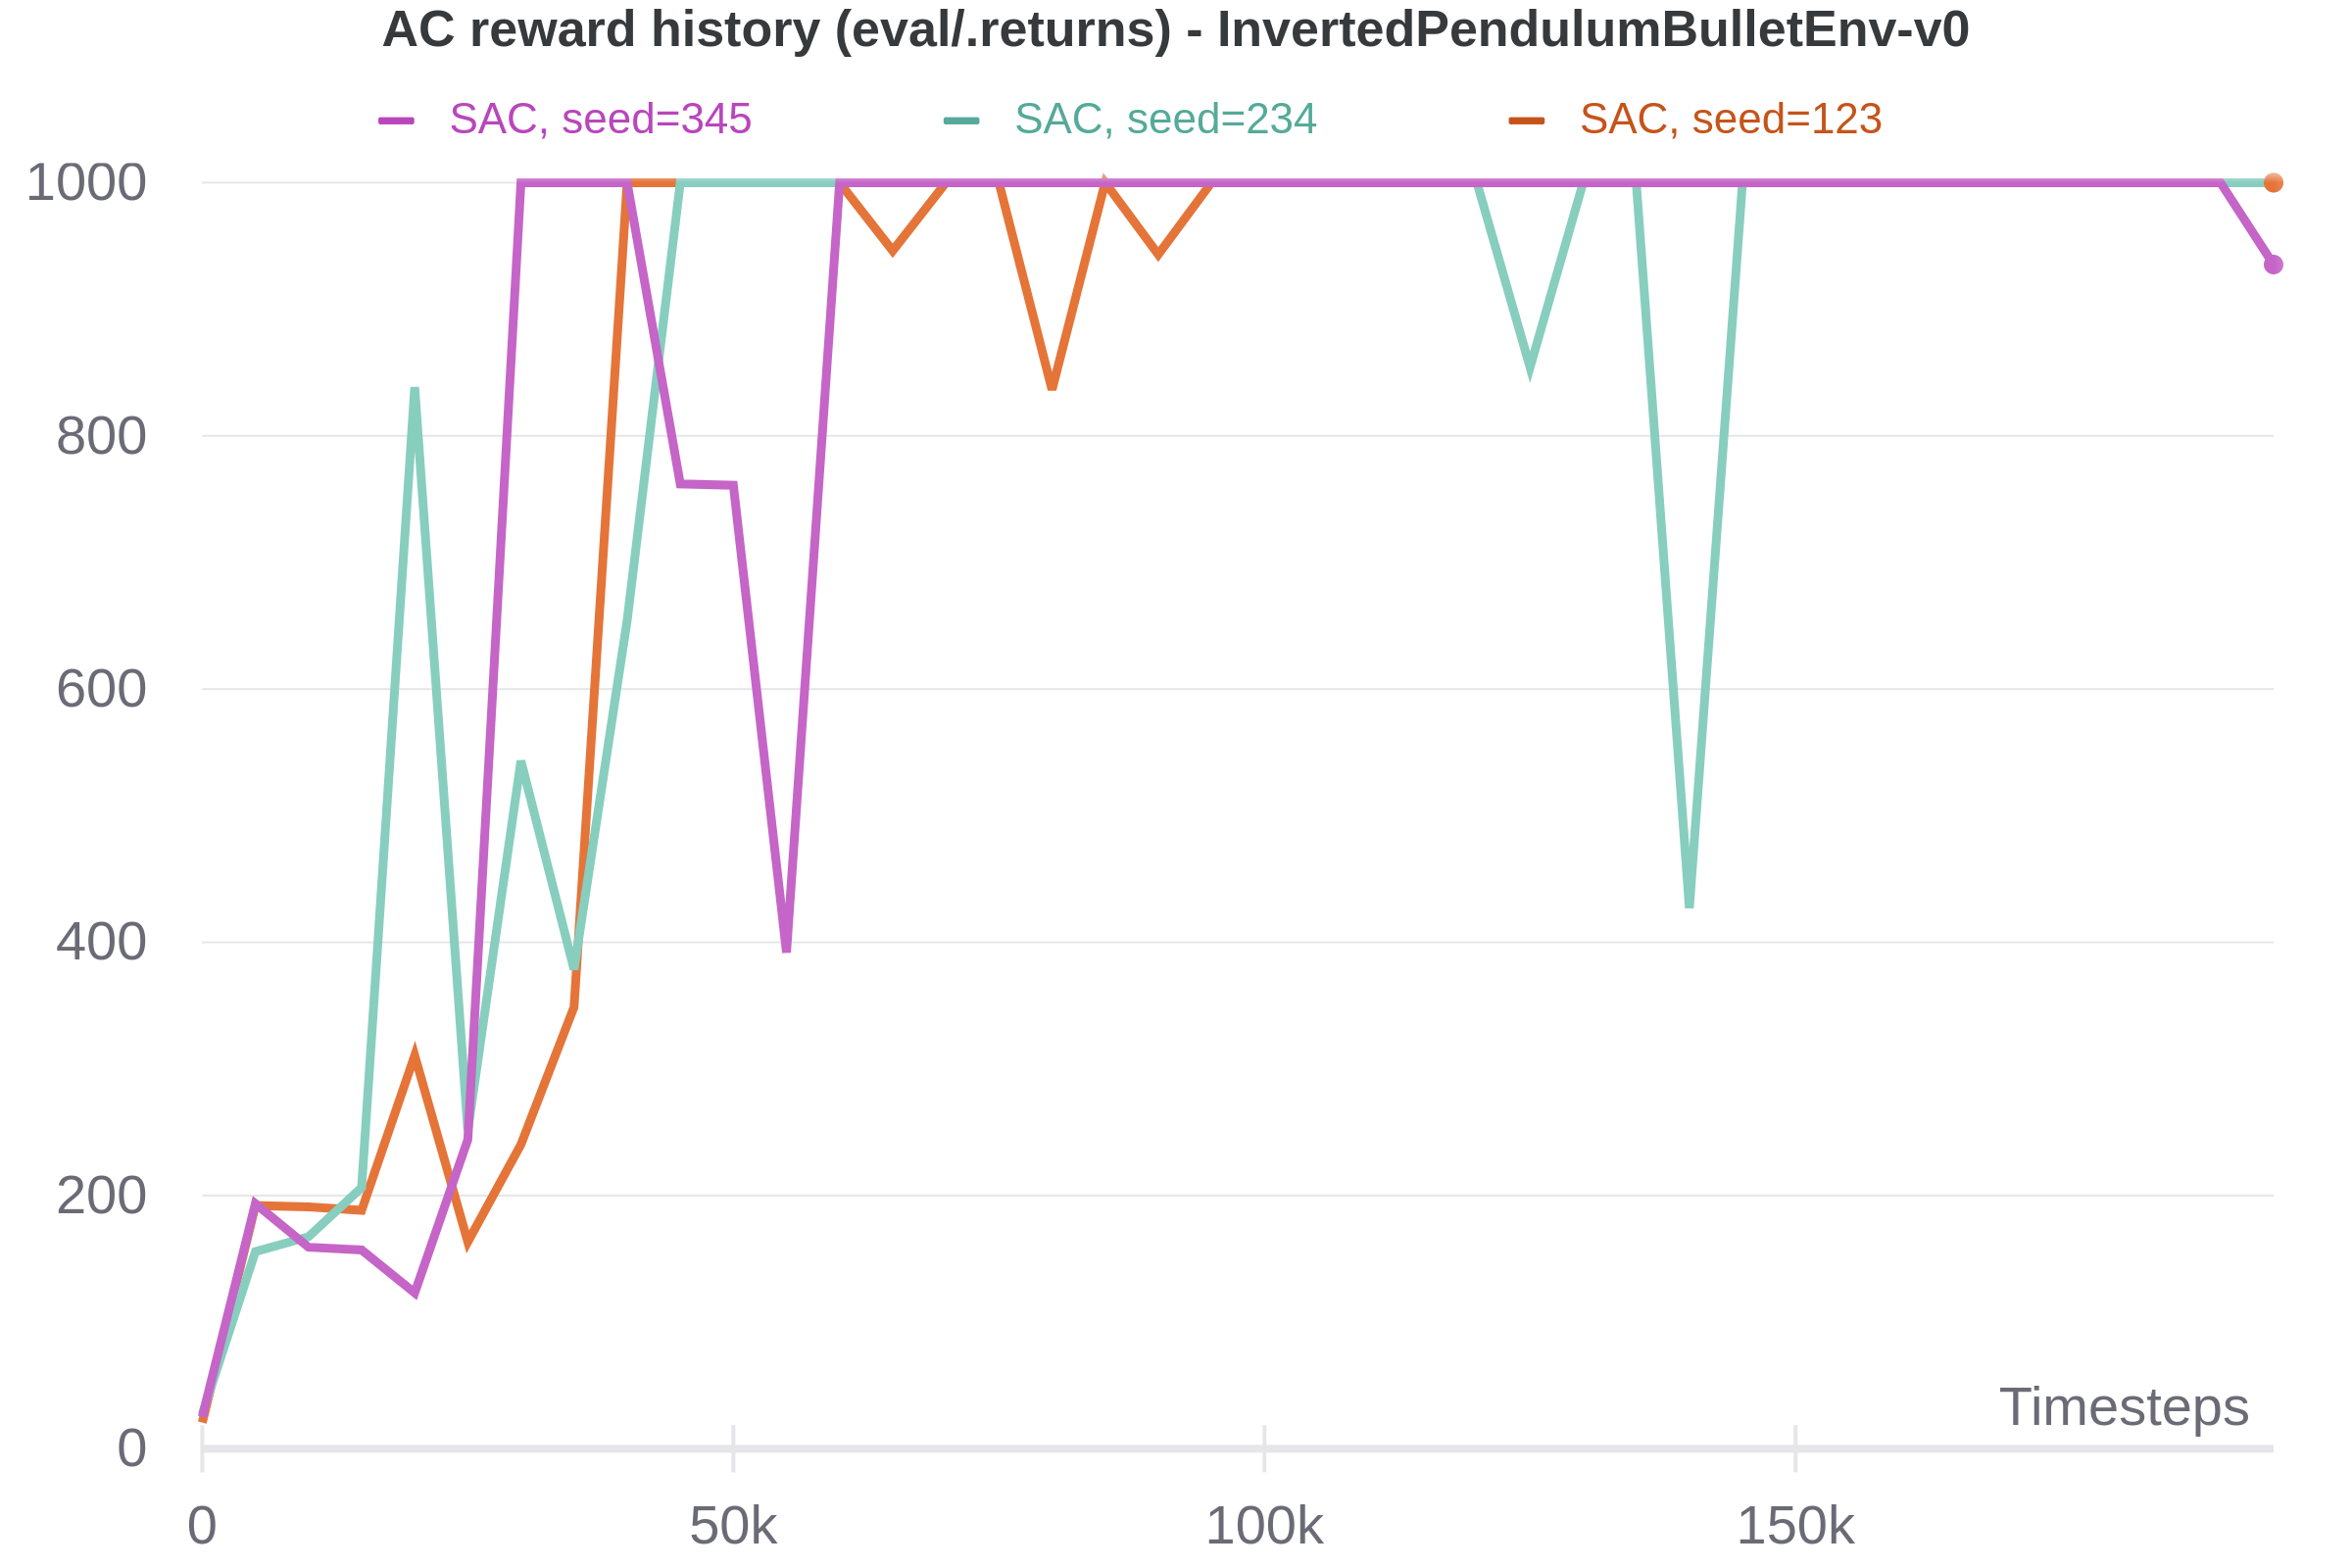
\includegraphics[width=0.65\columnwidth]{img/Figure_7_WB_InvertedPendulumBullet_SAC.png}
	\caption{Training performance of SAC algorithm in InvertedPendulumBullet environment.}
	\label{fig:fig7}
\end{figure}

\begin{figure}[phb] 
	\centering  % Remember to centre the figure
    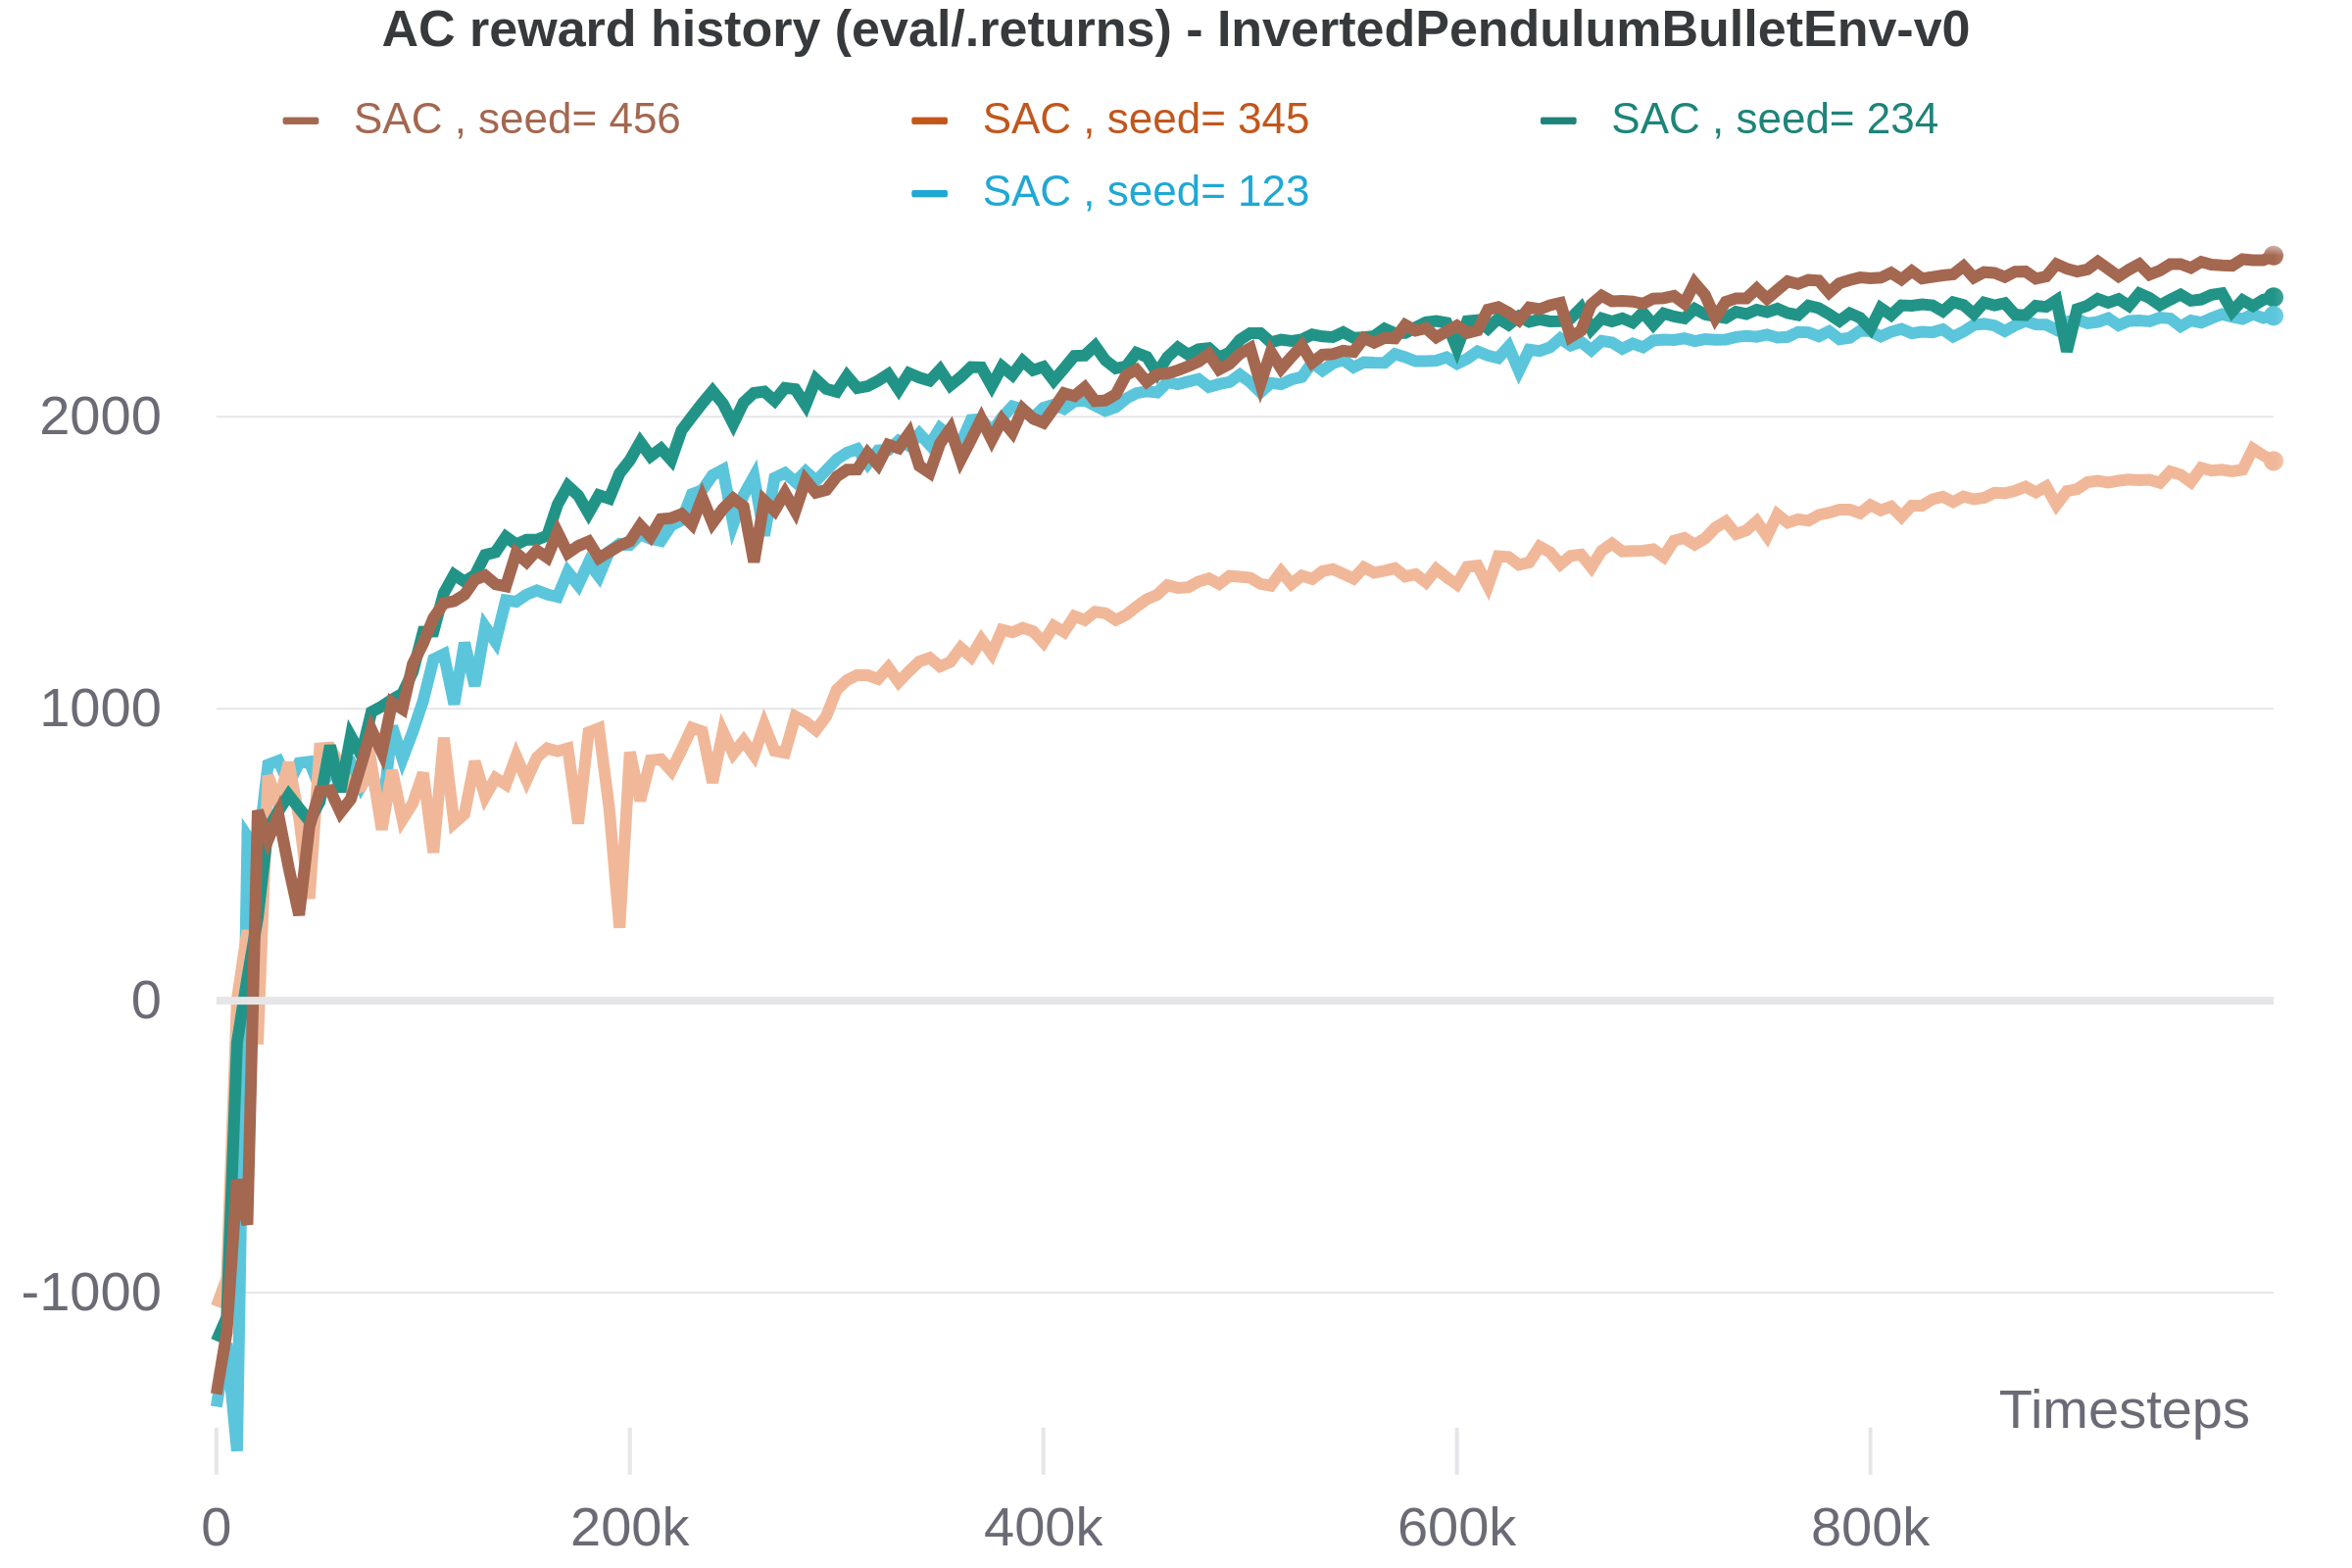
\includegraphics[width=0.65\columnwidth]{img/Figure_8_WB_HalfCheetahBullet_SAC.png}
	\caption{Training performance of SAC algorithm in HalfCheetahBullet environment.}
	\label{fig:fig8}
\end{figure}

\pagebreak

\begin{figure}[pht] 
	\centering  % Remember to centre the figure
    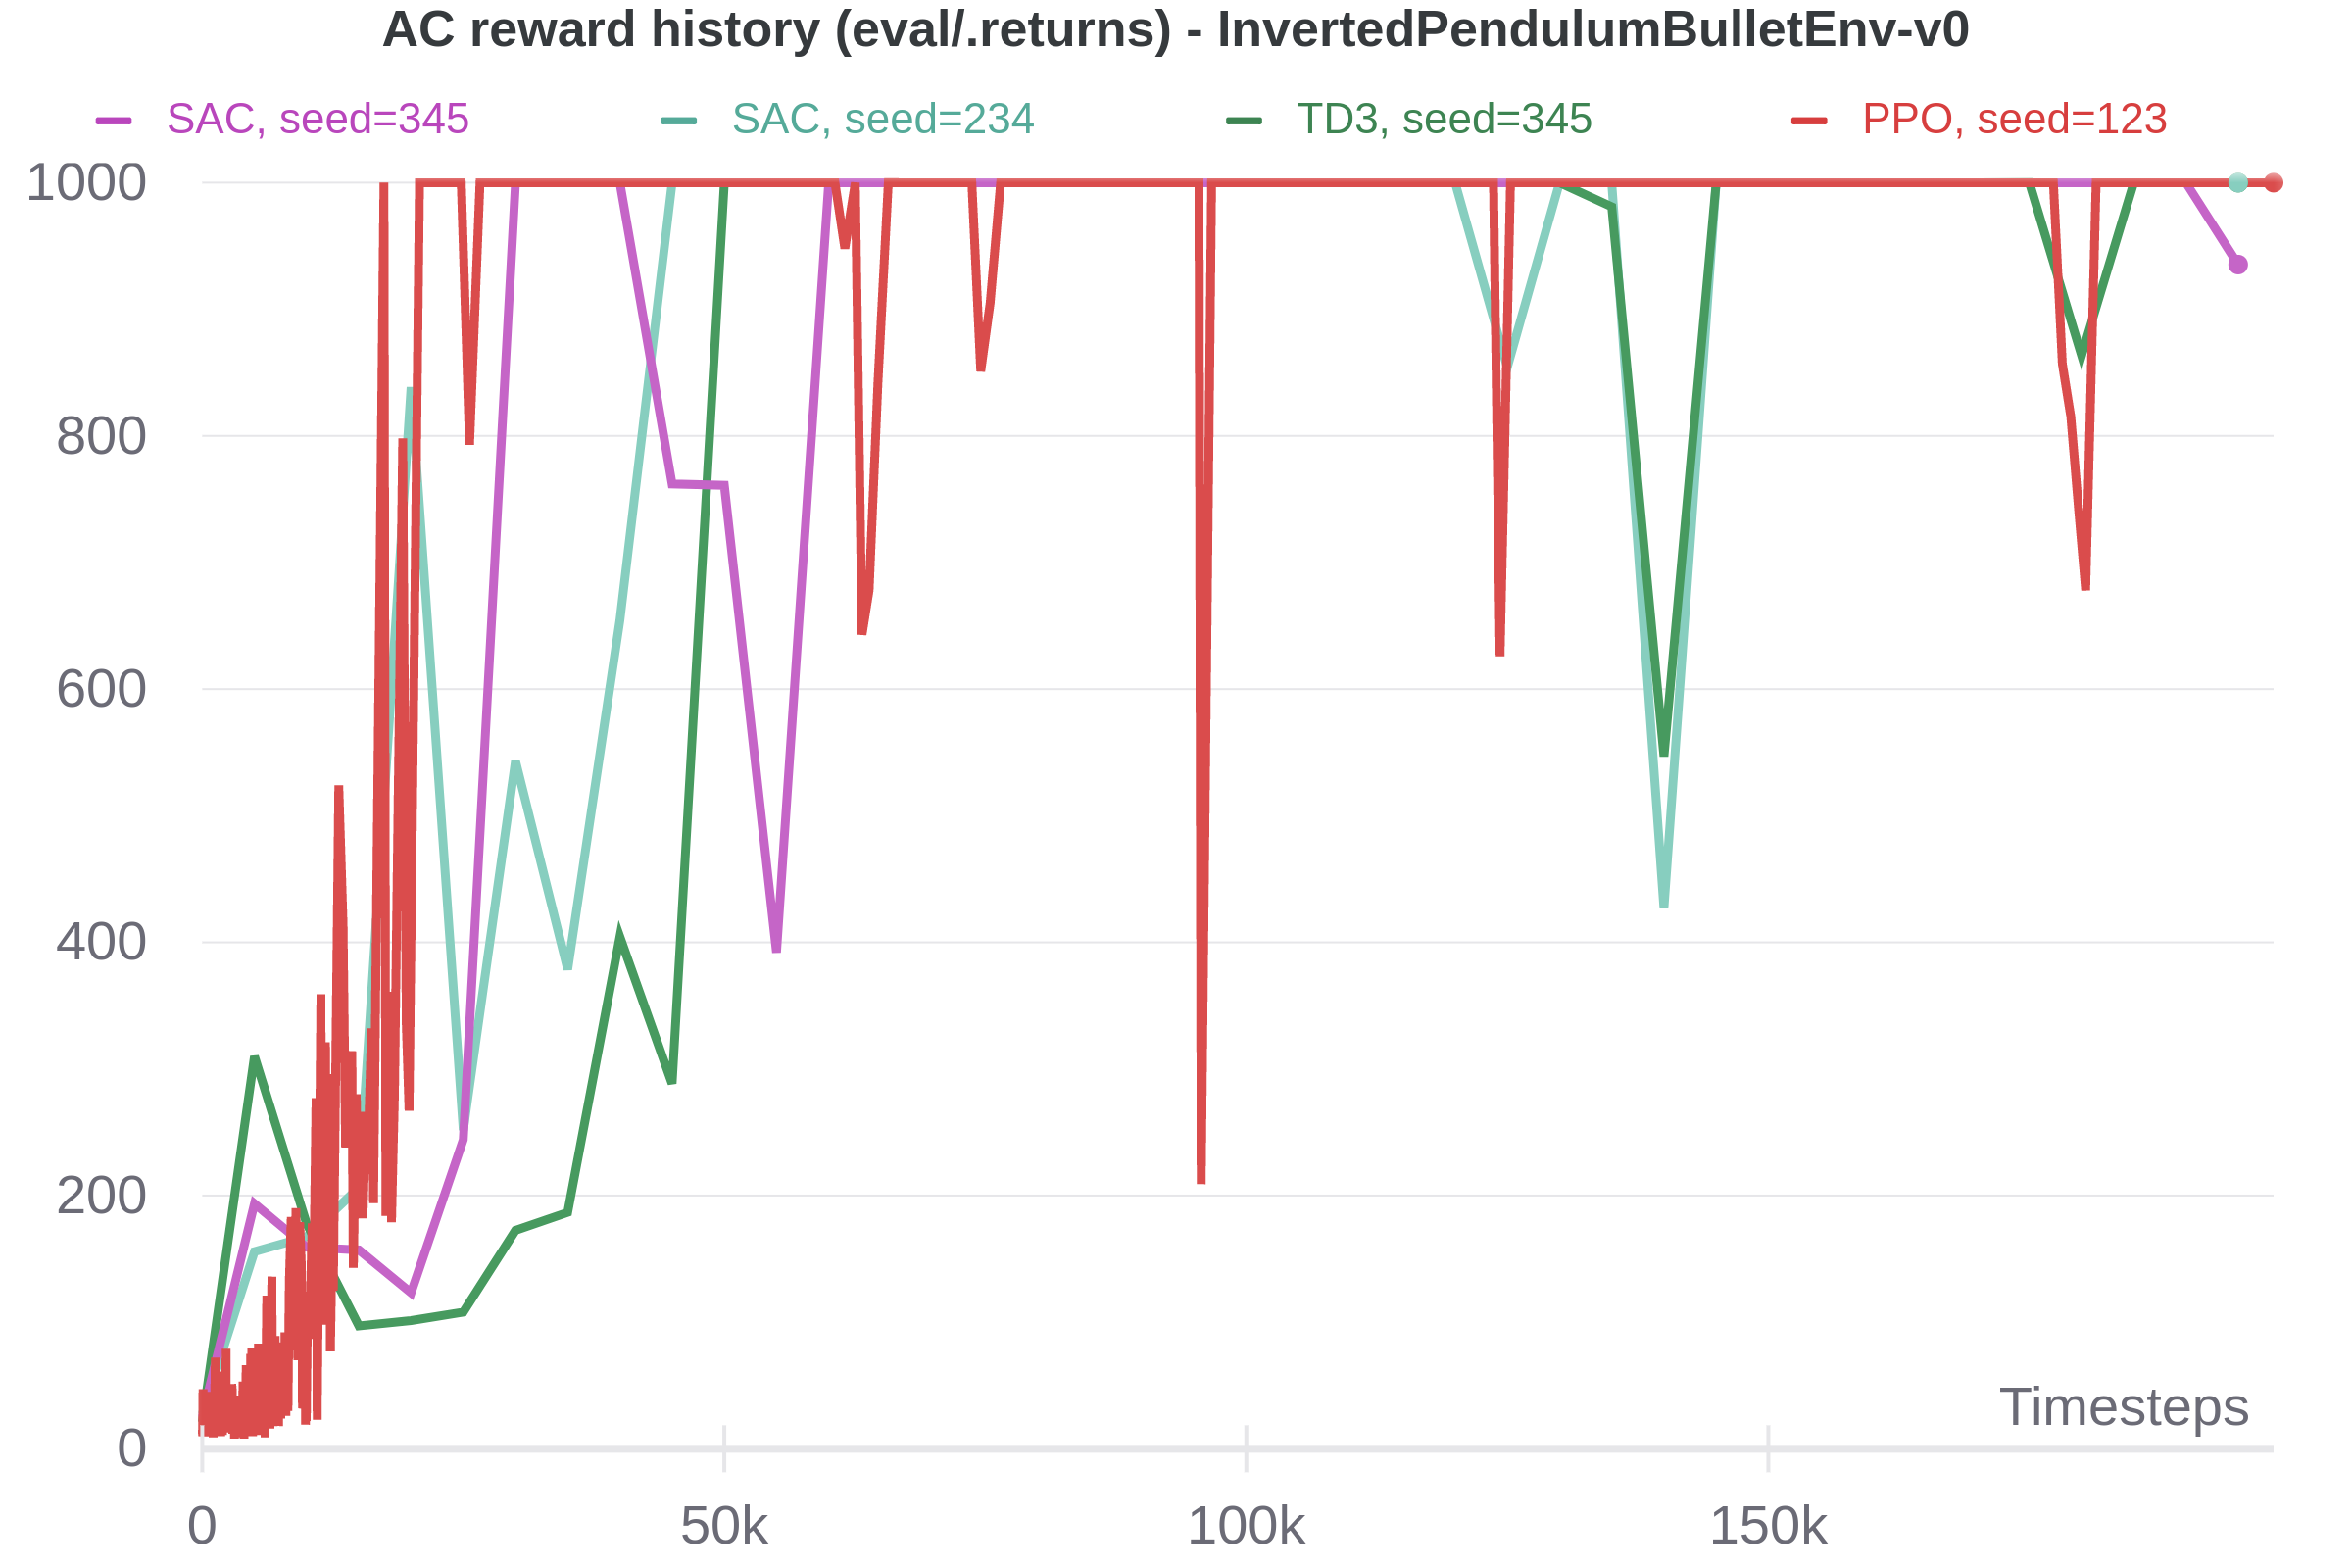
\includegraphics[width=0.65\columnwidth]{img/Figure_9_WB_InvertedPendulumBullet.png}
	\caption{Training performance of SAC, TD3, and PPO algorithms in InvertedPendulumBullet environment.}
	\label{fig:fig9}
\end{figure}

\begin{figure}[phb] 
	\centering  % Remember to centre the figure
    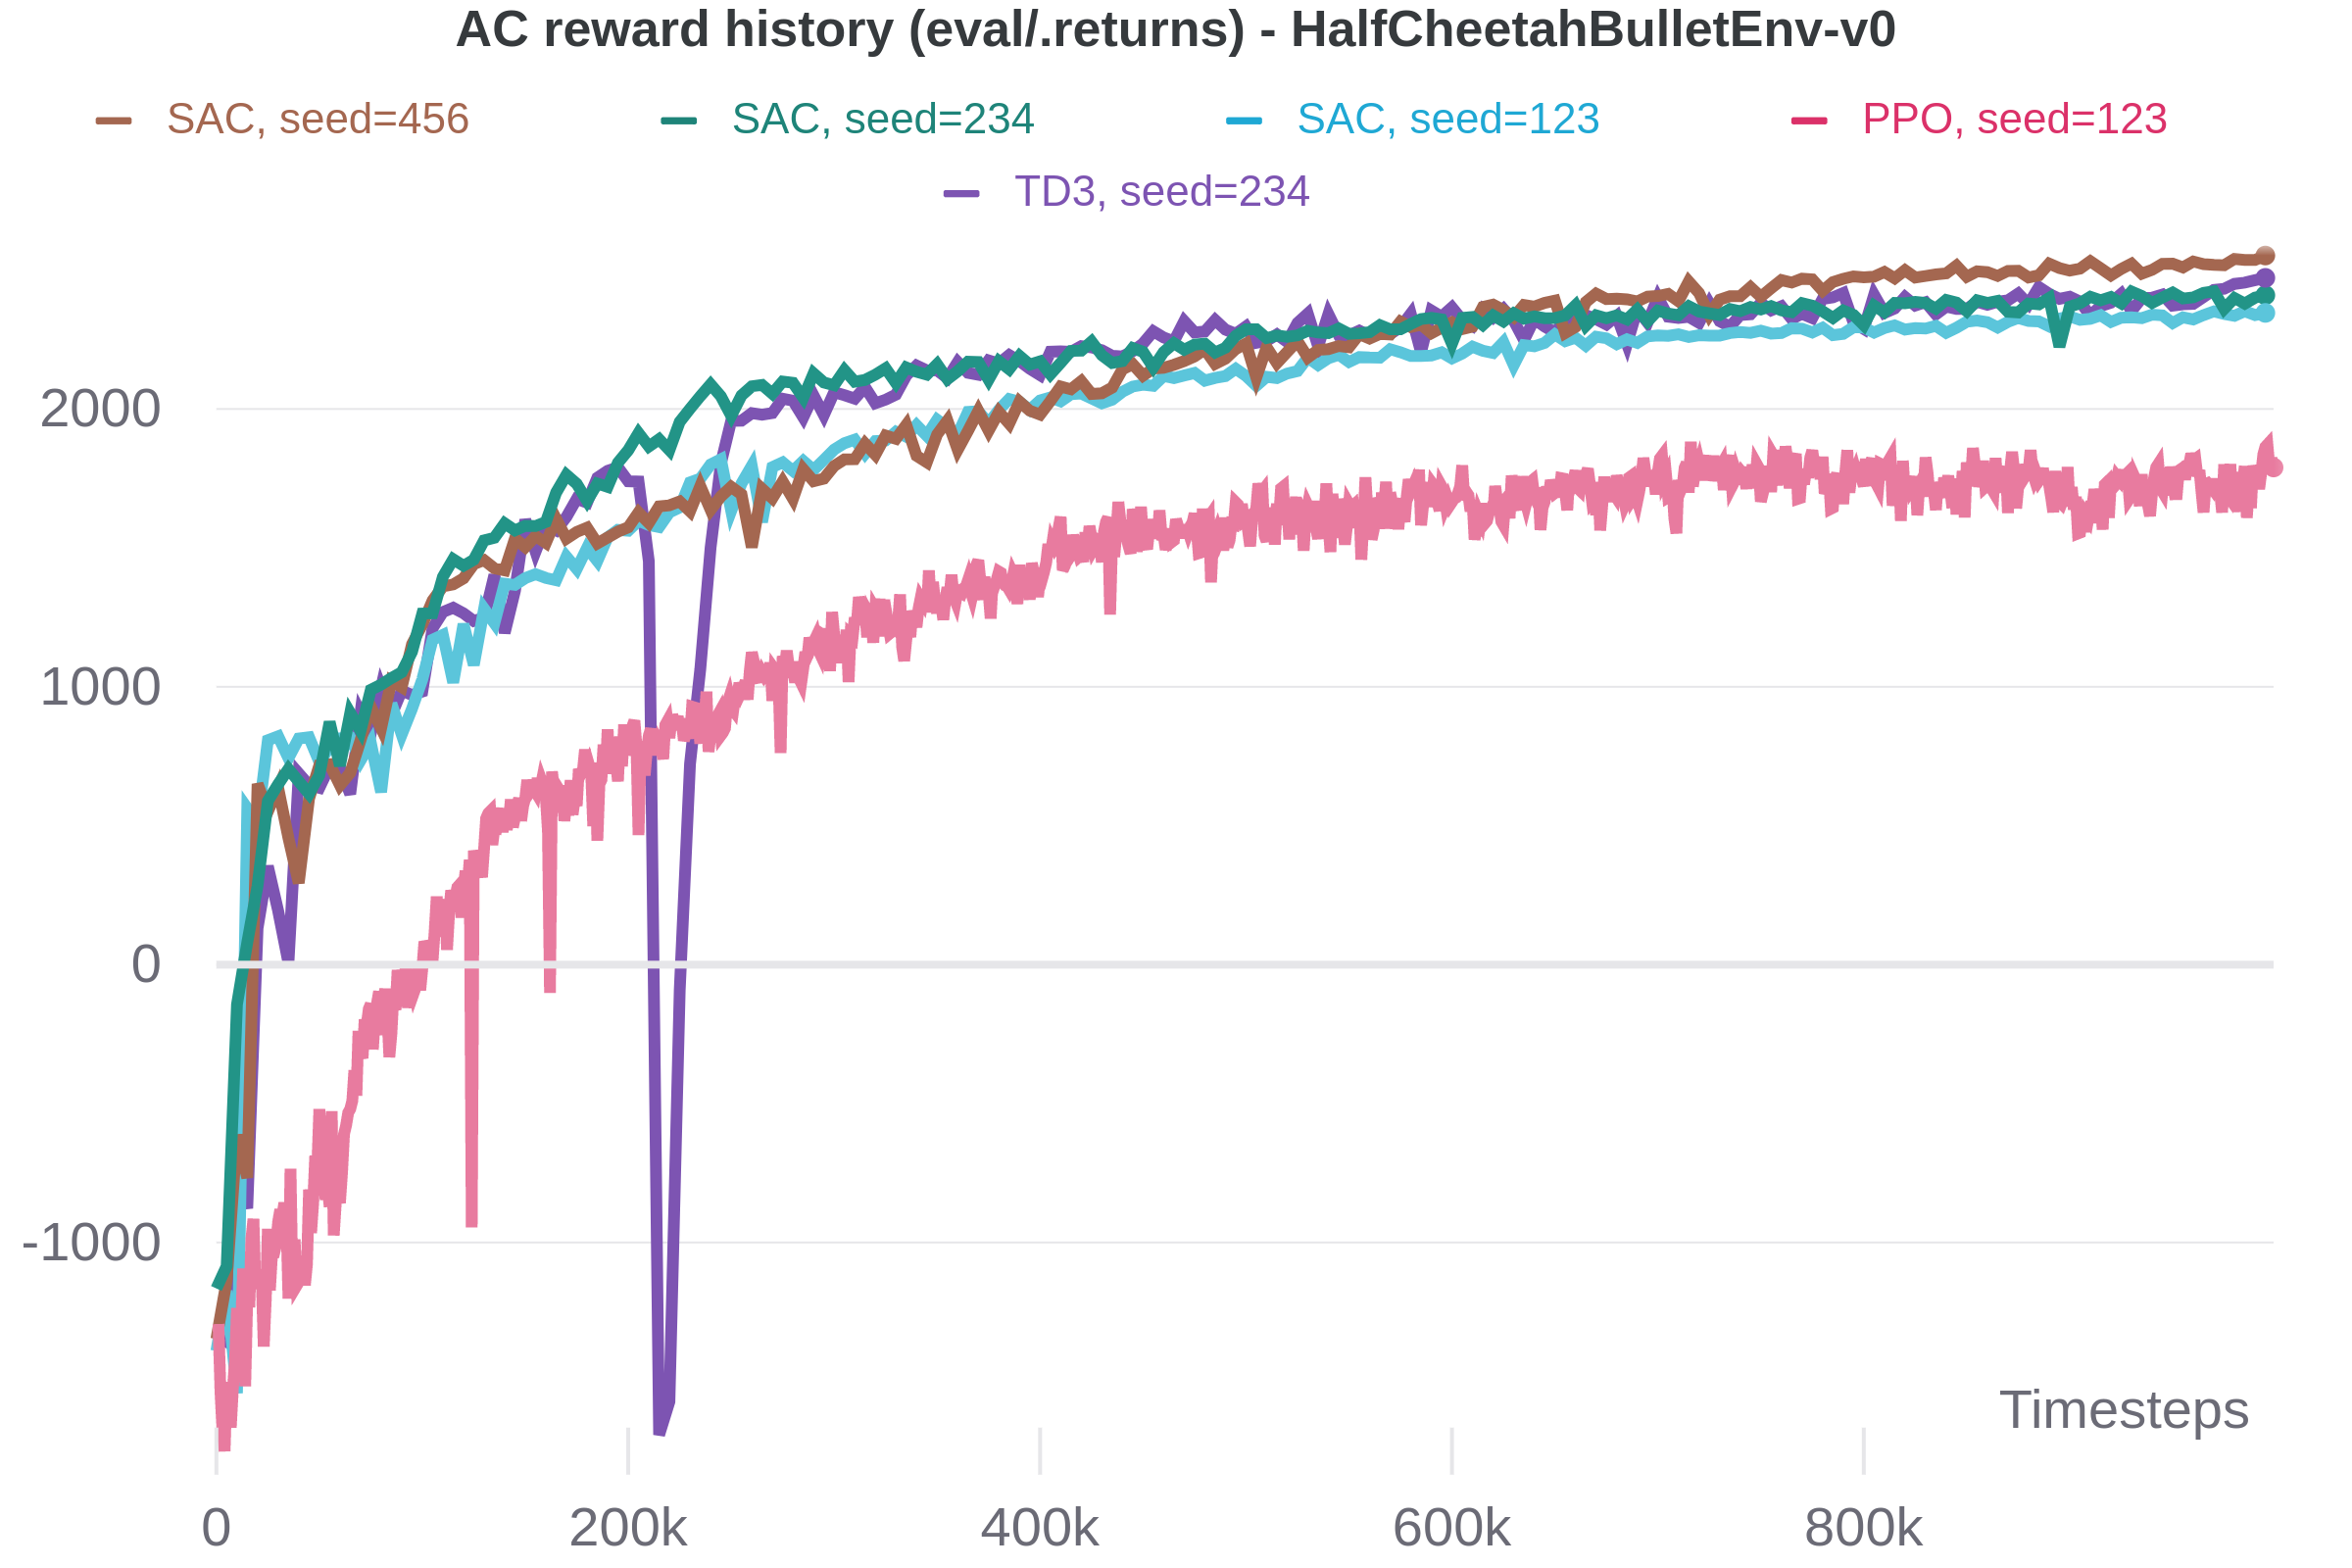
\includegraphics[width=0.65\columnwidth]{img/Figure_10_WB_HalfCheetahBullet.png}
	\caption{Training performance of SAC. TD3, and PPO algorithms in HalfCheetahBullet environment.}
	\label{fig:fig10}
\end{figure}

\pagebreak


\noindent
Also, you need to describe the network structure and training procedure as well
as hyperparemeters. A clear way to show the hyperparameters is using a table.

\subsection*{Question 2}

\noindent
Let’s analysis your algorithm by performing an ablation study. You could modify one design
option that you expect to influence the training performance. 
\newline

\noindent
Then train the agent using the modified code and compare the results to the original algorithm. Training your agent on HalfCheetah environment is enough but with three random seeds.
\newline

\subsection*{Hyperparameters}

qwmuq9wu9q8wuz98q
\newline

Table 1. SAC Hyperparameters
\begin{center}
\begin{tabular}{ l|l } 
 \hline
 Parameter & Value \\ 
 \hline\hline
 optimizer & Adam(Kingma \& Ba, 2015) \\ 
 learning rate & $3\cdot10^{-4}$ \\ 
 discount ($\gamma$) & 0.99 \\
 reply buffer size & $10^6$ \\
 number of hidden layers & 2 \\
 number of hidden units per layer & 256 \\
 number of samples per minibatch & 256 \\
 nonlinearity & ReLU \\
 \hline
\end{tabular}
\end{center}

Table 2. SAC Environment Specific Parameters
\begin{center}
\begin{tabular}{ l c c c } 
 \hline
 Environment & State Dimensions & Action Dimensions & Reward Scale \\ 
 \hline\hline
 InvertedPendulumBullet-v0 & 5 & 1 & 1 \\
 HalfCheetah-v0 & 26 & 6 & 5 \\ 
 \hline
\end{tabular}
\end{center}


\nocite{*}

\pagebreak

\section*{Conclusions}

\noindent
oekdwpodkwpod



\pagebreak



\bibliographystyle{ieeetr}
\bibliography{RL}  % Modify template with your bibliography name
\end{document}
